\documentclass[11pt]{article}

\usepackage[margin=1in]{geometry}
\usepackage[T1]{fontenc}
\usepackage[utf8]{inputenc}
\usepackage{lmodern}
\usepackage{microtype}
\usepackage{amsmath,amssymb,mathtools}
\usepackage{hyperref}
\usepackage{graphicx}
\usepackage{subcaption}
\usepackage{float}
\hypersetup{hidelinks}

\title{Short note on kernel GD experiments on $S^1$}
\author{Shreyas Kalvankar}
\date{\today}

\begin{document}
\maketitle

\section*{Summary}

These experiments support the following picture.

On the equally spaced circle grid, the kernel matrix is translation-invariant
and the Fourier modes decouple exactly. Hence kernel gradient descent can be
understood mode by mode:
\[
	r_k(t)=(1-\eta \lambda_k^{\mathrm{emp}})^t r_k(0).
\]
This gives a clean control experiment in which the role of amplitudes and
eigenvalues is fully transparent.

Within that exact setting, we observe two things. First, refining the grid from
$n=1024$ to $n=4096$ changes almost nothing: after normalization by $n$, the
empirical spectra match the continuum prediction very well, and the fitted
functions and normalized loss curves are nearly identical. Second, changing the
target amplitudes does not affect the decay rates. In particular, putting more mass in higher
modes makes the fit look worse at finite time because more residual "mass" sits
in high frequency, slow-fitting modes, not because the kernel dynamics themselves
changed.

Under i.i.d.\ uniform sampling, exact Fourier decoupling is lost, but the same
picture survives approximately. This is captured by the concentration of the
sampled Fourier geometry
\[
	G=\frac1n\Phi^\top\Phi,
\]
the compressed empirical operator
\[
	H=\frac1n\Phi^\top A_n\Phi,
\]
and the eigen-action error
\[
	E=A_n\Phi-\Phi\Lambda^{(n)}.
\]
Empirically, these quantities decrease with $n$ at the rates predicted by the finite-sample lemmas, which supports the claim that low Fourier modes remain approximately decoupled under random sampling.

\section*{1. Setup and exact mode dynamics on the equally spaced grid}

We first consider the equally spaced grid
\[
	\phi_j=\frac{2\pi j}{n}, \qquad j=0,\dots,n-1,
\]
and the cosine target
\[
	f^*(\phi)=\sum_{k=0}^3 \alpha_k \cos(k\phi).
\]
In the baseline experiment,
\[
	f^*(\phi)=1+0.9\cos(\phi)+0.5\cos(2\phi)+0.35\cos(3\phi).
\]

Let
\[
	K_{ij}=\Theta(\phi_i-\phi_j)
\]
be the raw kernel matrix and let
\[
	r_t := f_t-f^*
\]
denote the residual under kernel gradient descent
\[
	f_{t+1}=f_t-\eta K(f_t-f^*).
\]

Because the kernel is translation-invariant and the grid is equally spaced, the Fourier modes are exact eigenvectors of $K$. If
\[
	Kc_k=\lambda_k^{\mathrm{emp}}c_k,
\]
then the residual coefficient along mode $k$ evolves exactly as
\[
	r_k(t+1)=(1-\eta\lambda_k^{\mathrm{emp}})\,r_k(t),
	\qquad
	r_k(t)=(1-\eta\lambda_k^{\mathrm{emp}})^t r_k(0).
\]
For zero initialization,
\[
	r_k(0)=-\alpha_k,
	\qquad
	r_k(t)=-\alpha_k(1-\eta\lambda_k^{\mathrm{emp}})^t.
\]
Thus the amplitude $\alpha_k$ controls the initial size, while $\lambda_k^{\mathrm{emp}}$ controls the decay rate.

To compare decay rates independently of amplitudes, we normalize by the initial mode size:
\[
	\frac{|r_k(t)|}{|r_k(0)|}=|1-\eta\lambda_k^{\mathrm{emp}}|^t.
\]

The corresponding continuum operator is
\[
	(Tf)(\phi)=\int_0^{2\pi}\Theta(\phi-\psi)f(\psi)\,\frac{d\psi}{2\pi},
\]
with Fourier eigenvalues $\lambda_k^{\mathrm{cont}}$. Since the experiments above use the raw Gram matrix $K$, the equally spaced discretization satisfies
\[
	\lambda_k^{\mathrm{emp}} \approx n\,\lambda_k^{\mathrm{cont}}.
\]
Hence empirical eigenvalues should be divided by $n$ when compared across grid sizes or against the continuum prediction.

\section*{2. Exact-grid experiments}

\subsection*{2.1 Grid refinement: $n=1024$ versus $n=4096$}

We compare two equally spaced grid experiments:
\[
	\texttt{grid\_1024}: n=1024,
	\qquad
	\texttt{grid\_4096}: n=4096.
\]

\begin{figure}[H]
	\centering
	\begin{subfigure}[t]{0.48\textwidth}
		\centering
		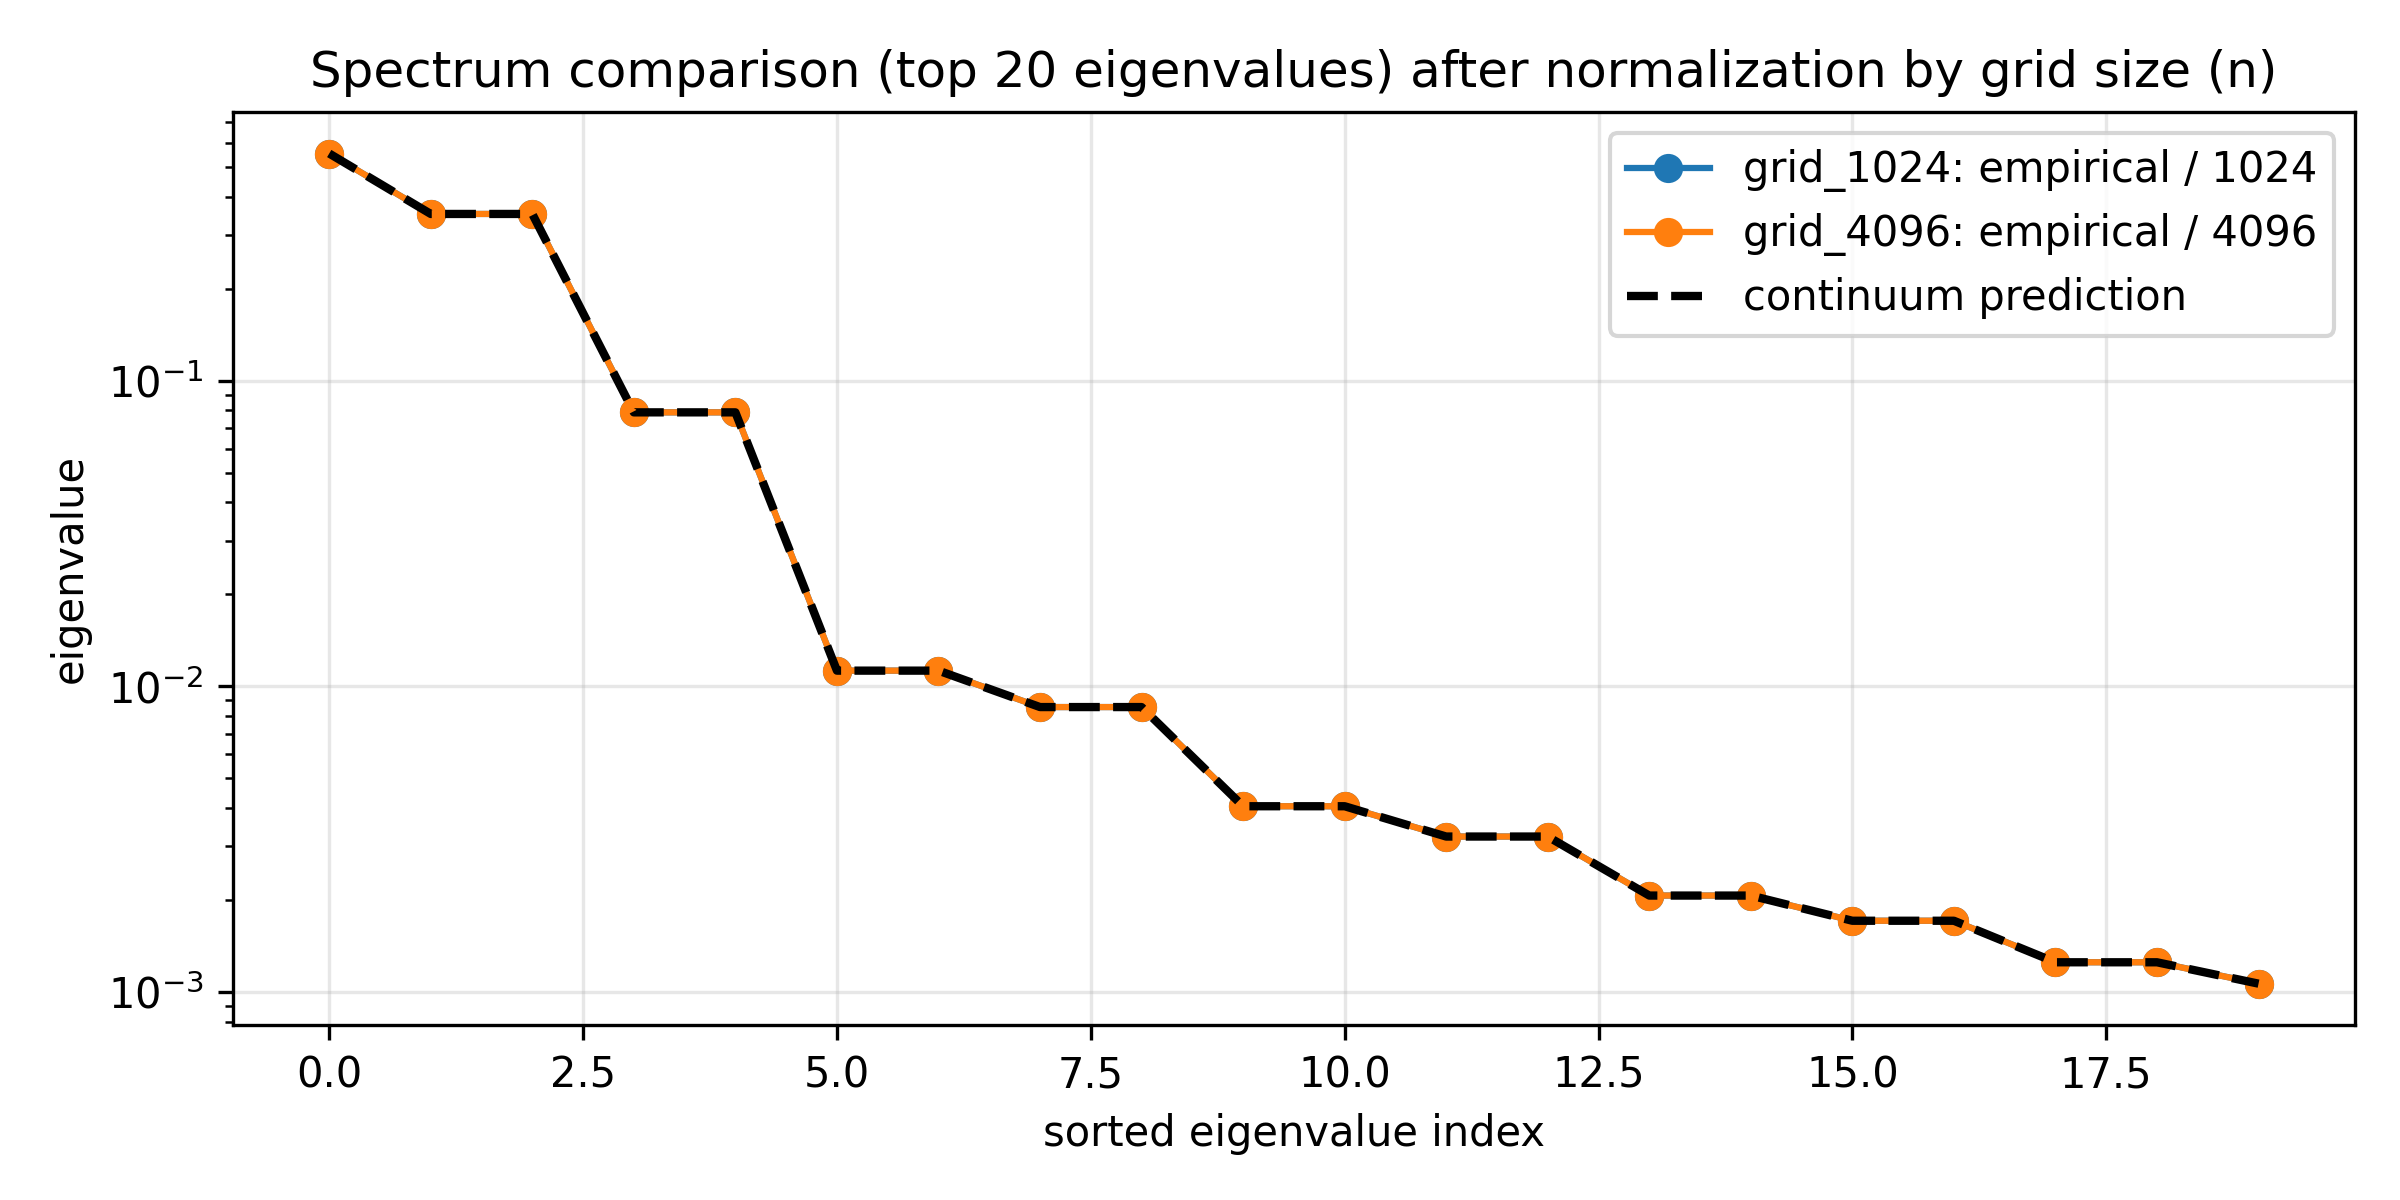
\includegraphics[width=\linewidth]{images/spectrum_comparison_grid.png}
		\caption{Top empirical eigenvalues after normalization by grid size.}
	\end{subfigure}
	\hfill
	\begin{subfigure}[t]{0.48\textwidth}
		\centering
		
\includegraphics[width=\linewidth]{images/loss_curve_grid.png}
		\caption{Residual decay normalized by grid size.}
	\end{subfigure}
	\caption{Grid refinement experiment. After normalization by $n$, the empirical spectra for $1024$ and $4096$ points almost coincide and both match the continuum prediction well. The normalized loss curves are also nearly identical.}
\end{figure}

This is the main control experiment. After dividing the empirical eigenvalues by $n$, the spectra for the two grids are visually indistinguishable and already close to the continuum values. Likewise, the normalized loss curves almost overlap. The conclusion is that the $1024$-point grid already captures the relevant low-frequency operator structure very accurately, so the remaining discrepancy in the slow modes is better explained by finite training time and numerical precision than by coarse discretization.

\subsection*{2.2 Amplitude swap: baseline versus high-frequency-heavy target}

We next keep the same equally spaced grid and kernel, but change only the target amplitudes:
\[
	\text{baseline: }
	f^*(\gamma)=1+0.9\cos(\gamma)+0.5\cos(2\gamma)+0.35\cos(3\gamma),
\]
\[
	\text{highfreq\_heavy: }
	f^*(\gamma)=1+0.35\cos(\gamma)+0.9\cos(2\gamma)+1.4\cos(3\gamma).
\]

The exact-grid formula predicts that changing amplitudes should not change the normalized mode decay rates, because the factor
\[
	(1-\eta\lambda_k^{\mathrm{emp}})^t
\]
depends only on the kernel spectrum, not on $\alpha_k$.

\begin{figure}[H]
	\centering
	\begin{subfigure}[t]{0.48\textwidth}
		\centering
		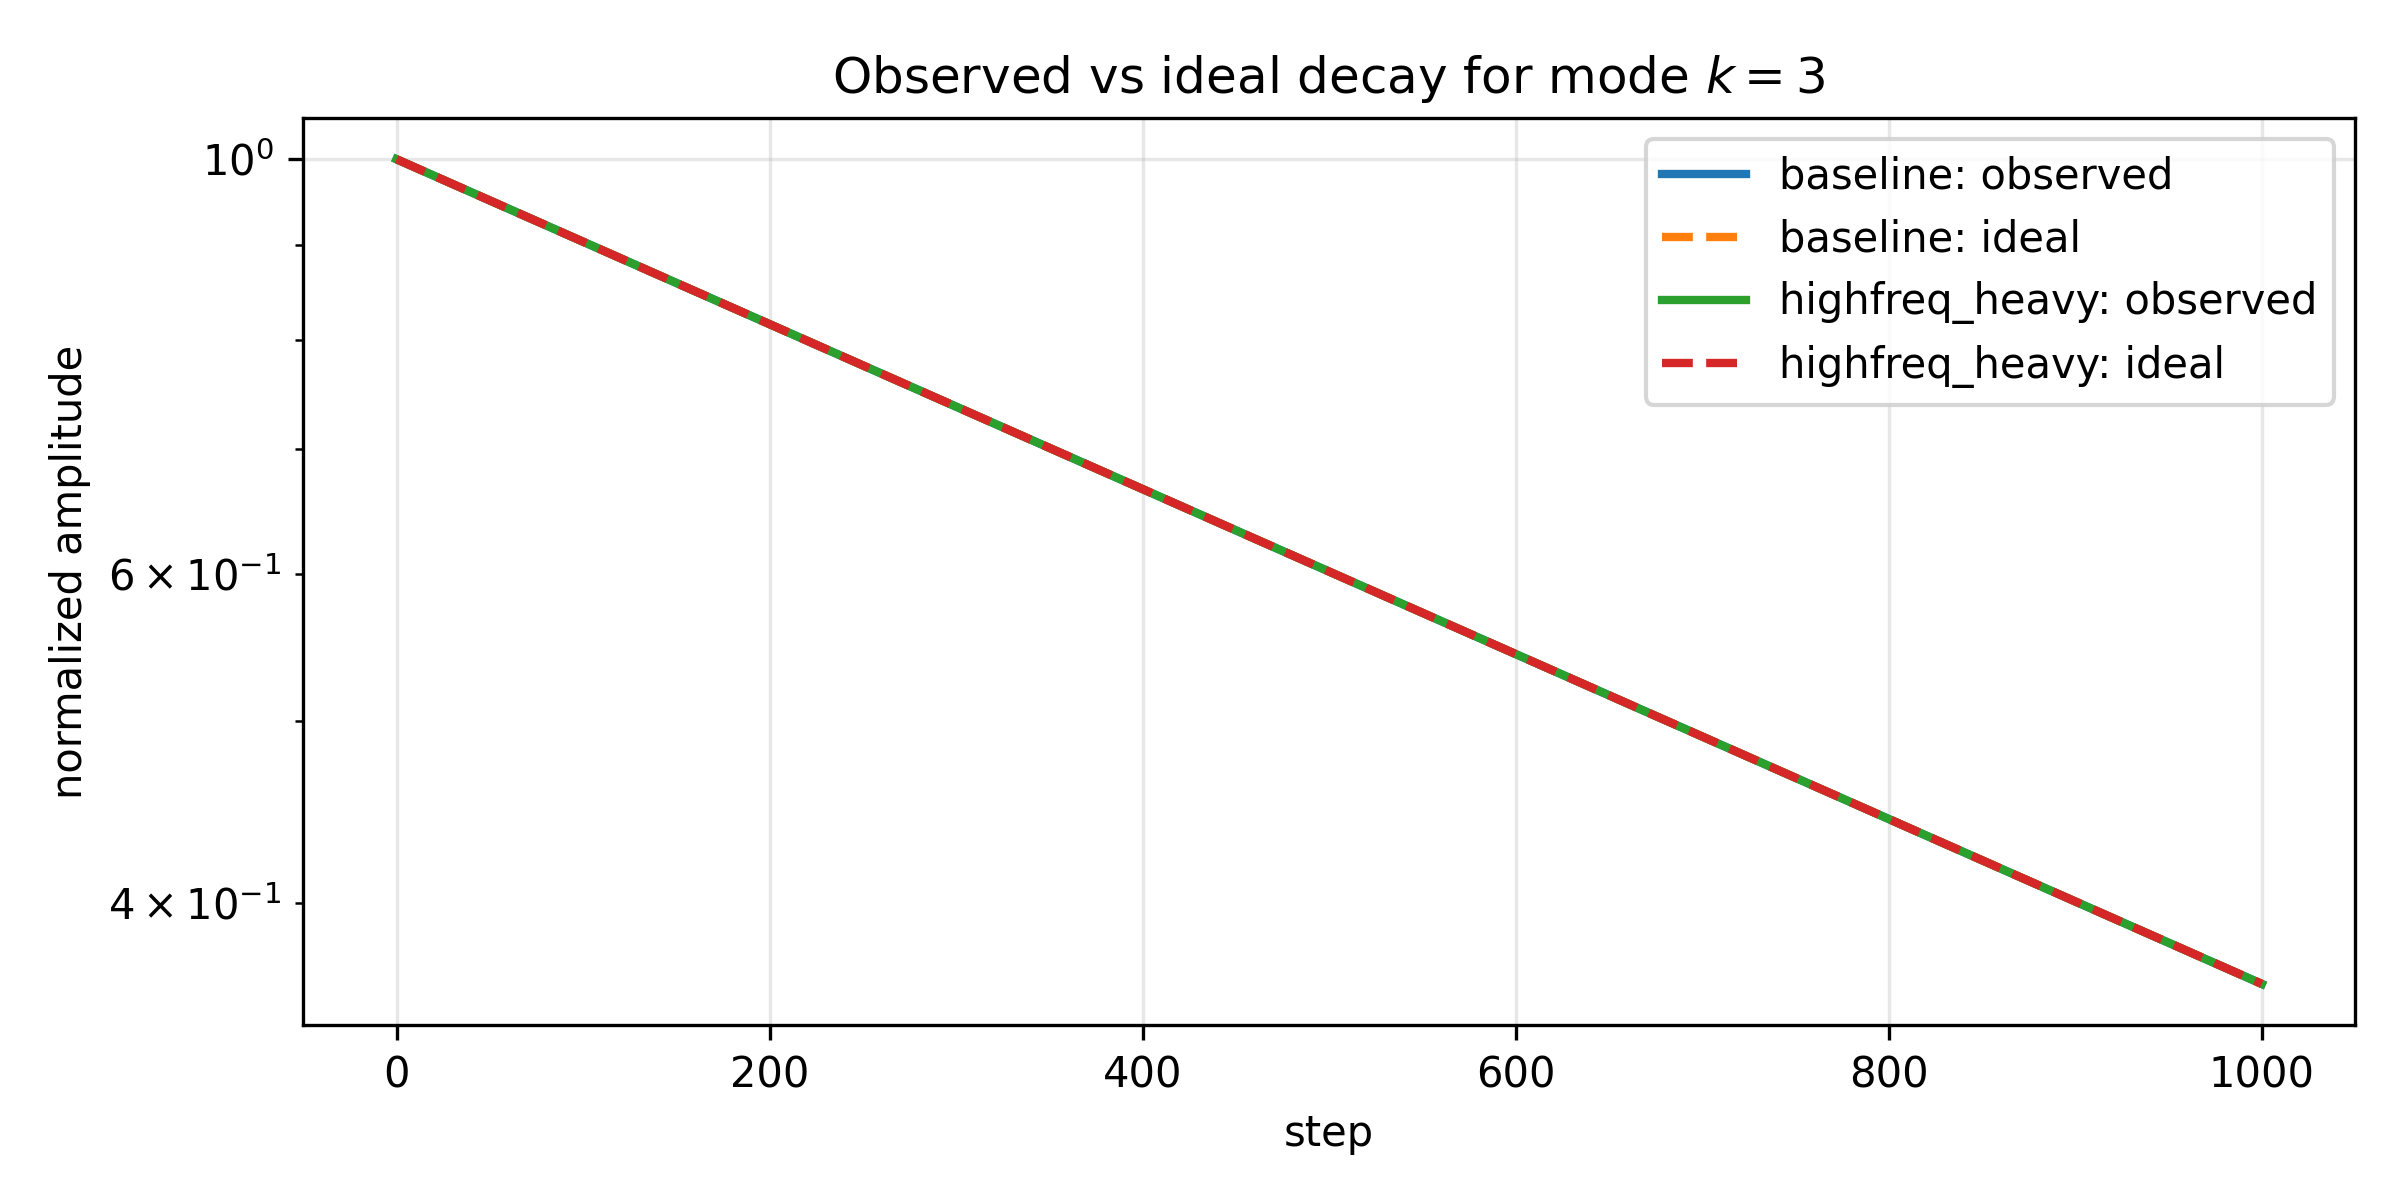
\includegraphics[width=\linewidth]{images/observed_vs_ideal_residual_decay_mode_3.png}
		\caption{Normalized residual decay, mode $k=3$.}
	\end{subfigure}
	\hfill
	\begin{subfigure}[t]{0.48\textwidth}
		\centering
		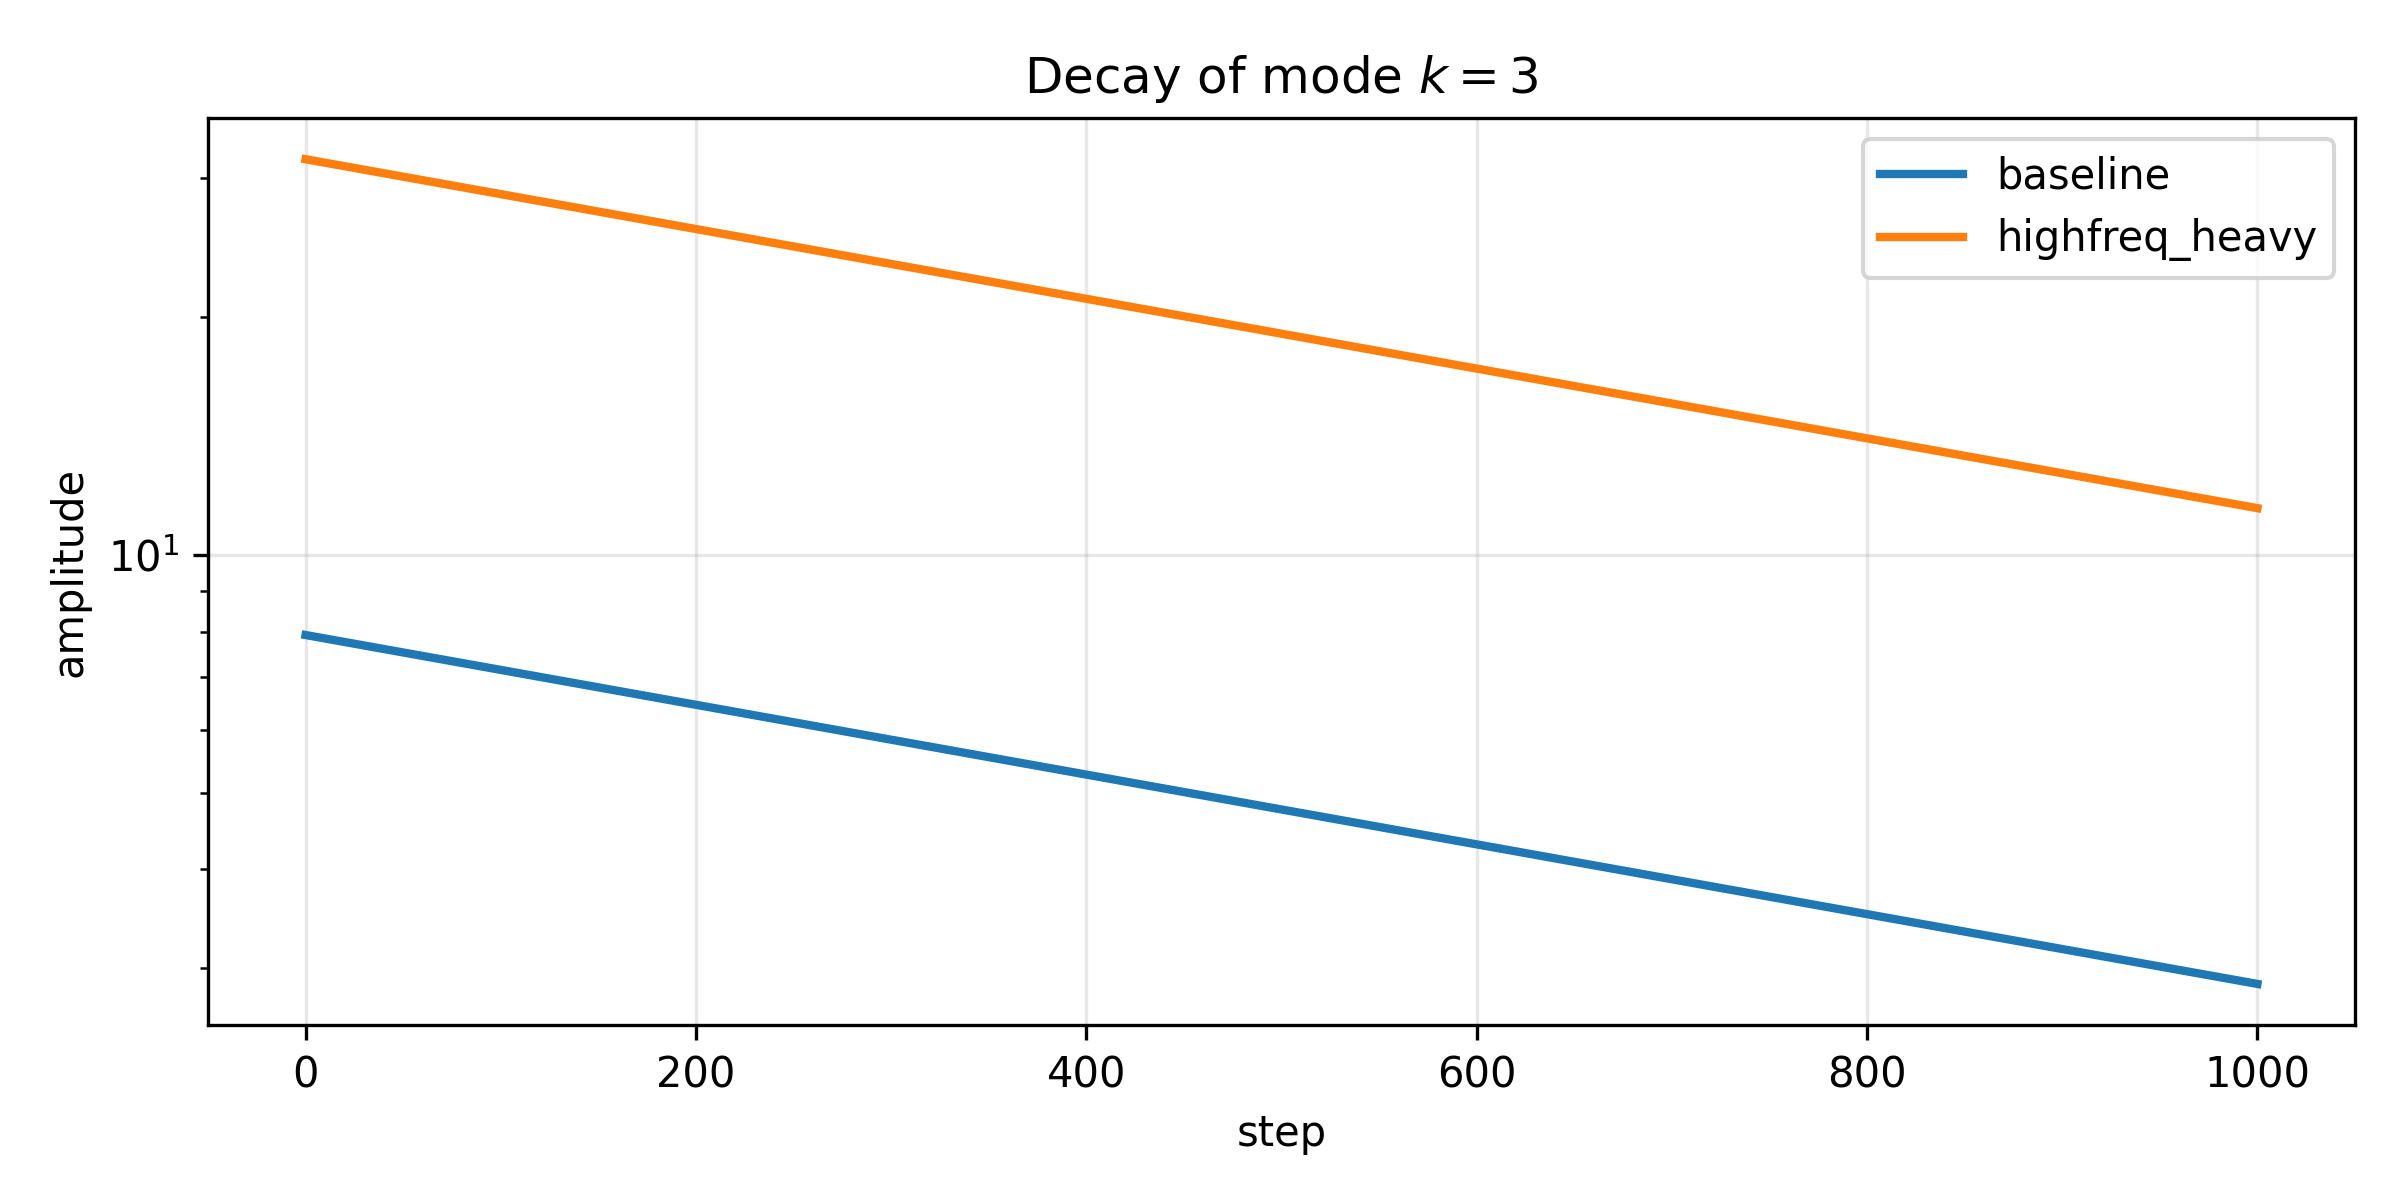
\includegraphics[width=\linewidth]{images/unnormalized_residual_decay_mode_3.png}
		\caption{Unnormalized residual decay, mode $k=3$.}
	\end{subfigure}
	\caption{Representative slow mode under the amplitude-swap experiment. The normalized curves coincide, confirming that the decay rate is unchanged. The unnormalized curves differ substantially because the initial mass in mode $k=3$ is much larger in the high-frequency-heavy target.}
\end{figure}

This is the key distinction. The normalized plots isolate the rate factor
\[
	(1-\eta\lambda_k^{\mathrm{emp}})^t,
\]
while the unnormalized plots retain the amplitude factor $\alpha_k$. Hence the high-frequency-heavy target looks harder to fit at finite time not because the mode-wise rates changed, but because more of the initial residual energy is concentrated in slow modes.

Equivalently, for zero initialization,
\[
	r_k(t)=-\alpha_k(1-\eta\lambda_k^{\mathrm{emp}})^t.
\]
So amplitudes change the absolute contribution of a mode to the residual, but not its decay rate.

\section*{3. Approximate decoupling under random sampling}

The equally spaced grid gives an exact Fourier-diagonal model of kernel gradient descent. Under i.i.d.\ uniform sampling, this exact structure is lost. The right question is therefore whether it survives approximately on the low-frequency Fourier block.

We now sample
\[
	\phi_1,\dots,\phi_n \overset{\mathrm{iid}}{\sim} \mathrm{Unif}[0,2\pi),
\]
define the empirical operator
\[
	(A_n v)_i=\frac1n\sum_{j=1}^n \Theta(\phi_i,\phi_j)\,v_j,
\]
and let
\[
	\Phi\in\mathbb{R}^{n\times d}
\]
be the sampled Fourier feature matrix for the low-frequency modes up to some fixed cutoff $K_{\max}$.

The three key finite-sample objects are
\[
	G=\frac1n\Phi^\top\Phi,
	\qquad
	H=\frac1n\Phi^\top A_n\Phi,
	\qquad
	E=A_n\Phi-\Phi\Lambda^{(n)},
\]
where
\[
	\lambda_k^{(n)}=\left(1-\frac1n\right)\lambda_k+\frac1n g(0),
	\qquad
	g(0)=\Theta(0).
\]

These have a direct interpretation:
\begin{itemize}
	\item $G\approx I$ means the sampled Fourier vectors remain nearly orthonormal,
	\item $H\approx \Lambda^{(n)}$ means the empirical operator is nearly diagonal on the low-frequency Fourier block,
	\item $E\approx 0$ means the sampled Fourier modes are approximate empirical eigenvectors.
\end{itemize}

If this holds, then low-mode residual coefficients should evolve approximately as
\[
	\alpha_k(t+1)\approx (1-\eta\lambda_k^{(n)})\alpha_k(t),
\]
so the exact mode picture from the equally spaced grid survives in approximate form.

\section*{4. Finite-sample concentration and lemma validation}

The finite-sample lemmas give exponential tail bounds in the deviation size $\varepsilon$ at fixed $n$, not exponential decay of the plotted errors in $n$. Solving these tail bounds for $\varepsilon$ yields the concentration scales
\[
	\|G-I\|_{\max}\sim n^{-1/2},
	\qquad
	\|H-\Lambda^{(n)}\|_{\max}\sim n^{-1/2},
	\qquad
	\|A_n\Phi-\Phi\Lambda^{(n)}\|_{\max}\sim \sqrt{\frac{\log n}{n}},
\]
up to constants and lower-order logarithmic factors.

\begin{figure}[H]
	\centering

	\begin{subfigure}[t]{0.48\textwidth}
		\centering
		
\includegraphics[width=\textwidth]{lemma_images/concentration_plot_gram_err_max.png}
		\caption{$\|G-I\|_{\max}$}
	\end{subfigure}
	\hfill
	\begin{subfigure}[t]{0.48\textwidth}
		\centering
		
\includegraphics[width=\textwidth]{lemma_images/concentration_plot_comp_err_max.png}
		\caption{$\|H-\Lambda^{(n)}\|_{\max}$}
	\end{subfigure}

	\vspace{0.8em}

	\begin{subfigure}[t]{0.62\textwidth}
		\centering
		
\includegraphics[width=\textwidth]{lemma_images/concentration_plot_action_err_max.png}
		\caption{$\|A_n\Phi-\Phi\Lambda^{(n)}\|_{\max}$}
	\end{subfigure}

	\caption{Finite-sample lemma validation under uniform sampling. The empirical errors decrease with $n$ and track the predicted rates well: $n^{-1/2}$ for the Gram and compressed-operator errors, and $\sqrt{\log n / n}$ for the action error.}
\end{figure}

As $n$ increases, the sampled Fourier block becomes better
conditioned, the empirical operator becomes more nearly diagonal on that block,
and the sampled Fourier modes behave more like approximate eigenvectors. This
is exactly the structure needed to justify approximate low-mode decoupling of
kernel gradient descent under random sampling.

\section*{5. Main takeaways}

\begin{enumerate}
	\item On the equally spaced grid, the Fourier picture is exact, and the experiments closely follow the formula
	      \[
		      r_k(t)=(1-\eta\lambda_k^{\mathrm{emp}})^t r_k(0).
	      \]

	\item The grid-refinement experiment suggests that the $1024$-point equally spaced grid is already a very accurate discretization for the low modes relevant here.

	\item The amplitude-swap experiment cleanly separates \emph{rate} from
	      \emph{size}: amplitudes change the error in absolute value, but not the mode-wise decay rates.

	\item Under i.i.d.\ uniform sampling, exact decoupling is replaced by approximate decoupling, and the numerical experiments support the predicted concentration of
	      \[
		      G,\quad H,\quad A_n\Phi-\Phi\Lambda^{(n)}.
	      \]
\end{enumerate}

\clearpage
\appendix
\section*{Supplementary plots}

This section collects the remaining plots that support the main discussion but were omitted from the body to keep the note short.

\subsection*{A. Additional plots for the grid-refinement experiment}

These plots provide the remaining evidence for the claim that increasing the equally spaced grid from $1024$ to $4096$ does not materially change the fit, the final error profile, or the mode-wise decay behavior.

\begin{figure}[H]
	\centering
	\begin{subfigure}[t]{0.48\textwidth}
		\centering
		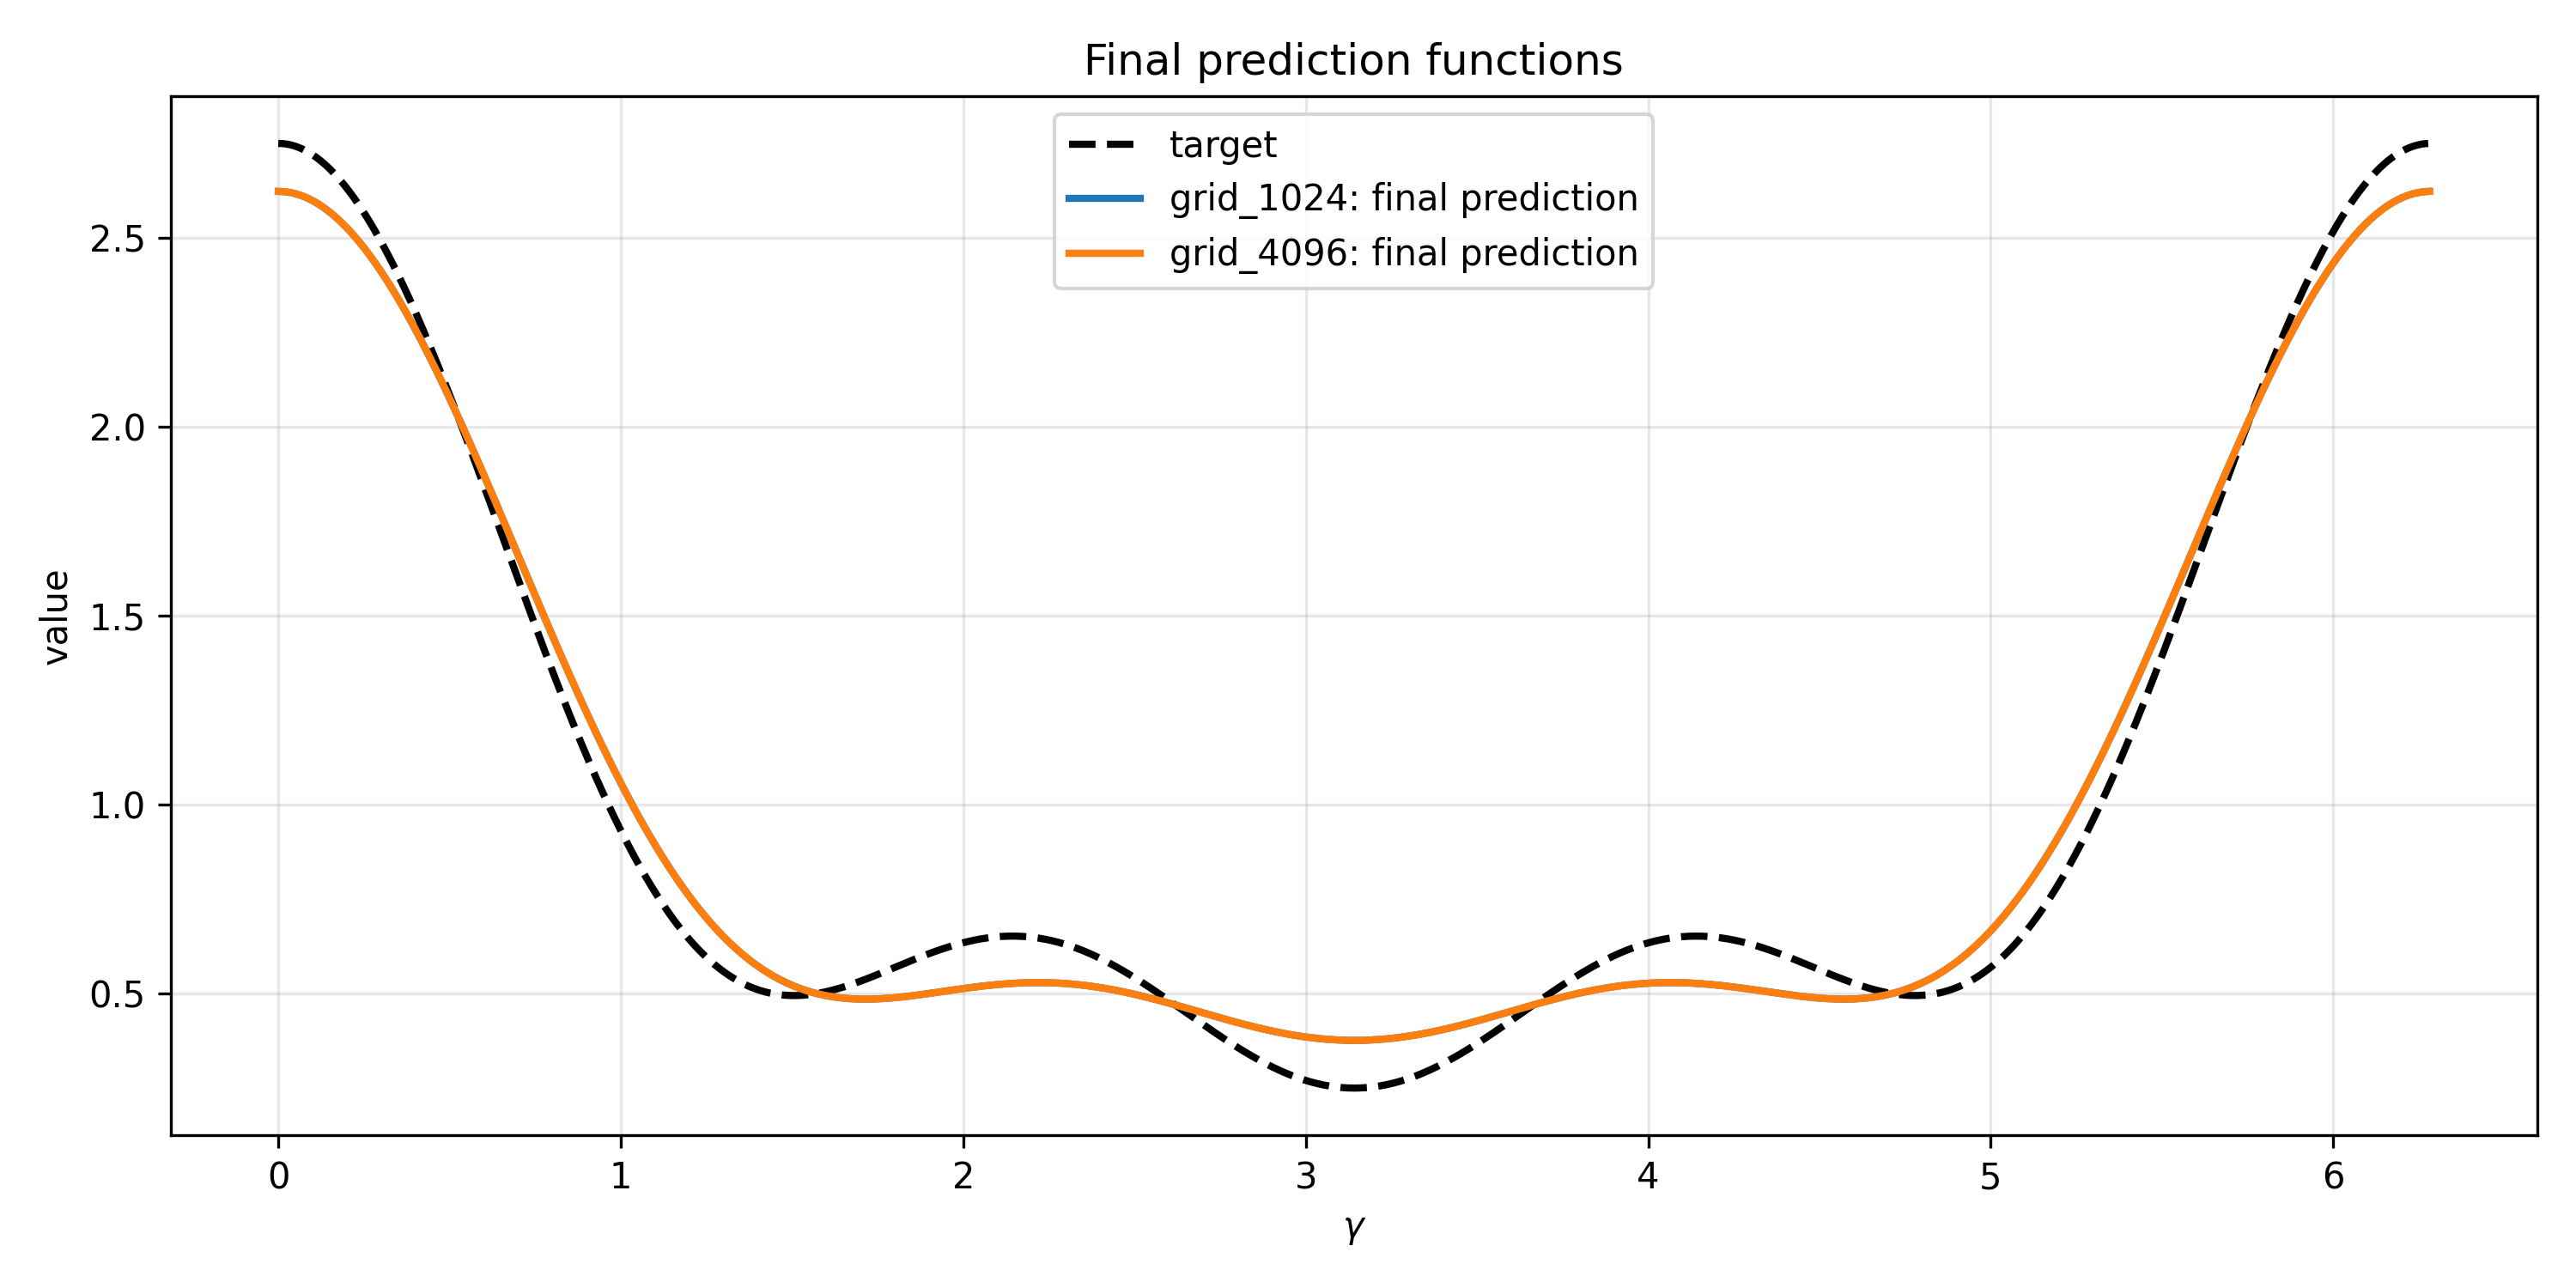
\includegraphics[width=\linewidth]{images/final_predictions_grid.png}
		\caption{Final prediction functions}
	\end{subfigure}
	\hfill
	\begin{subfigure}[t]{0.48\textwidth}
		\centering
		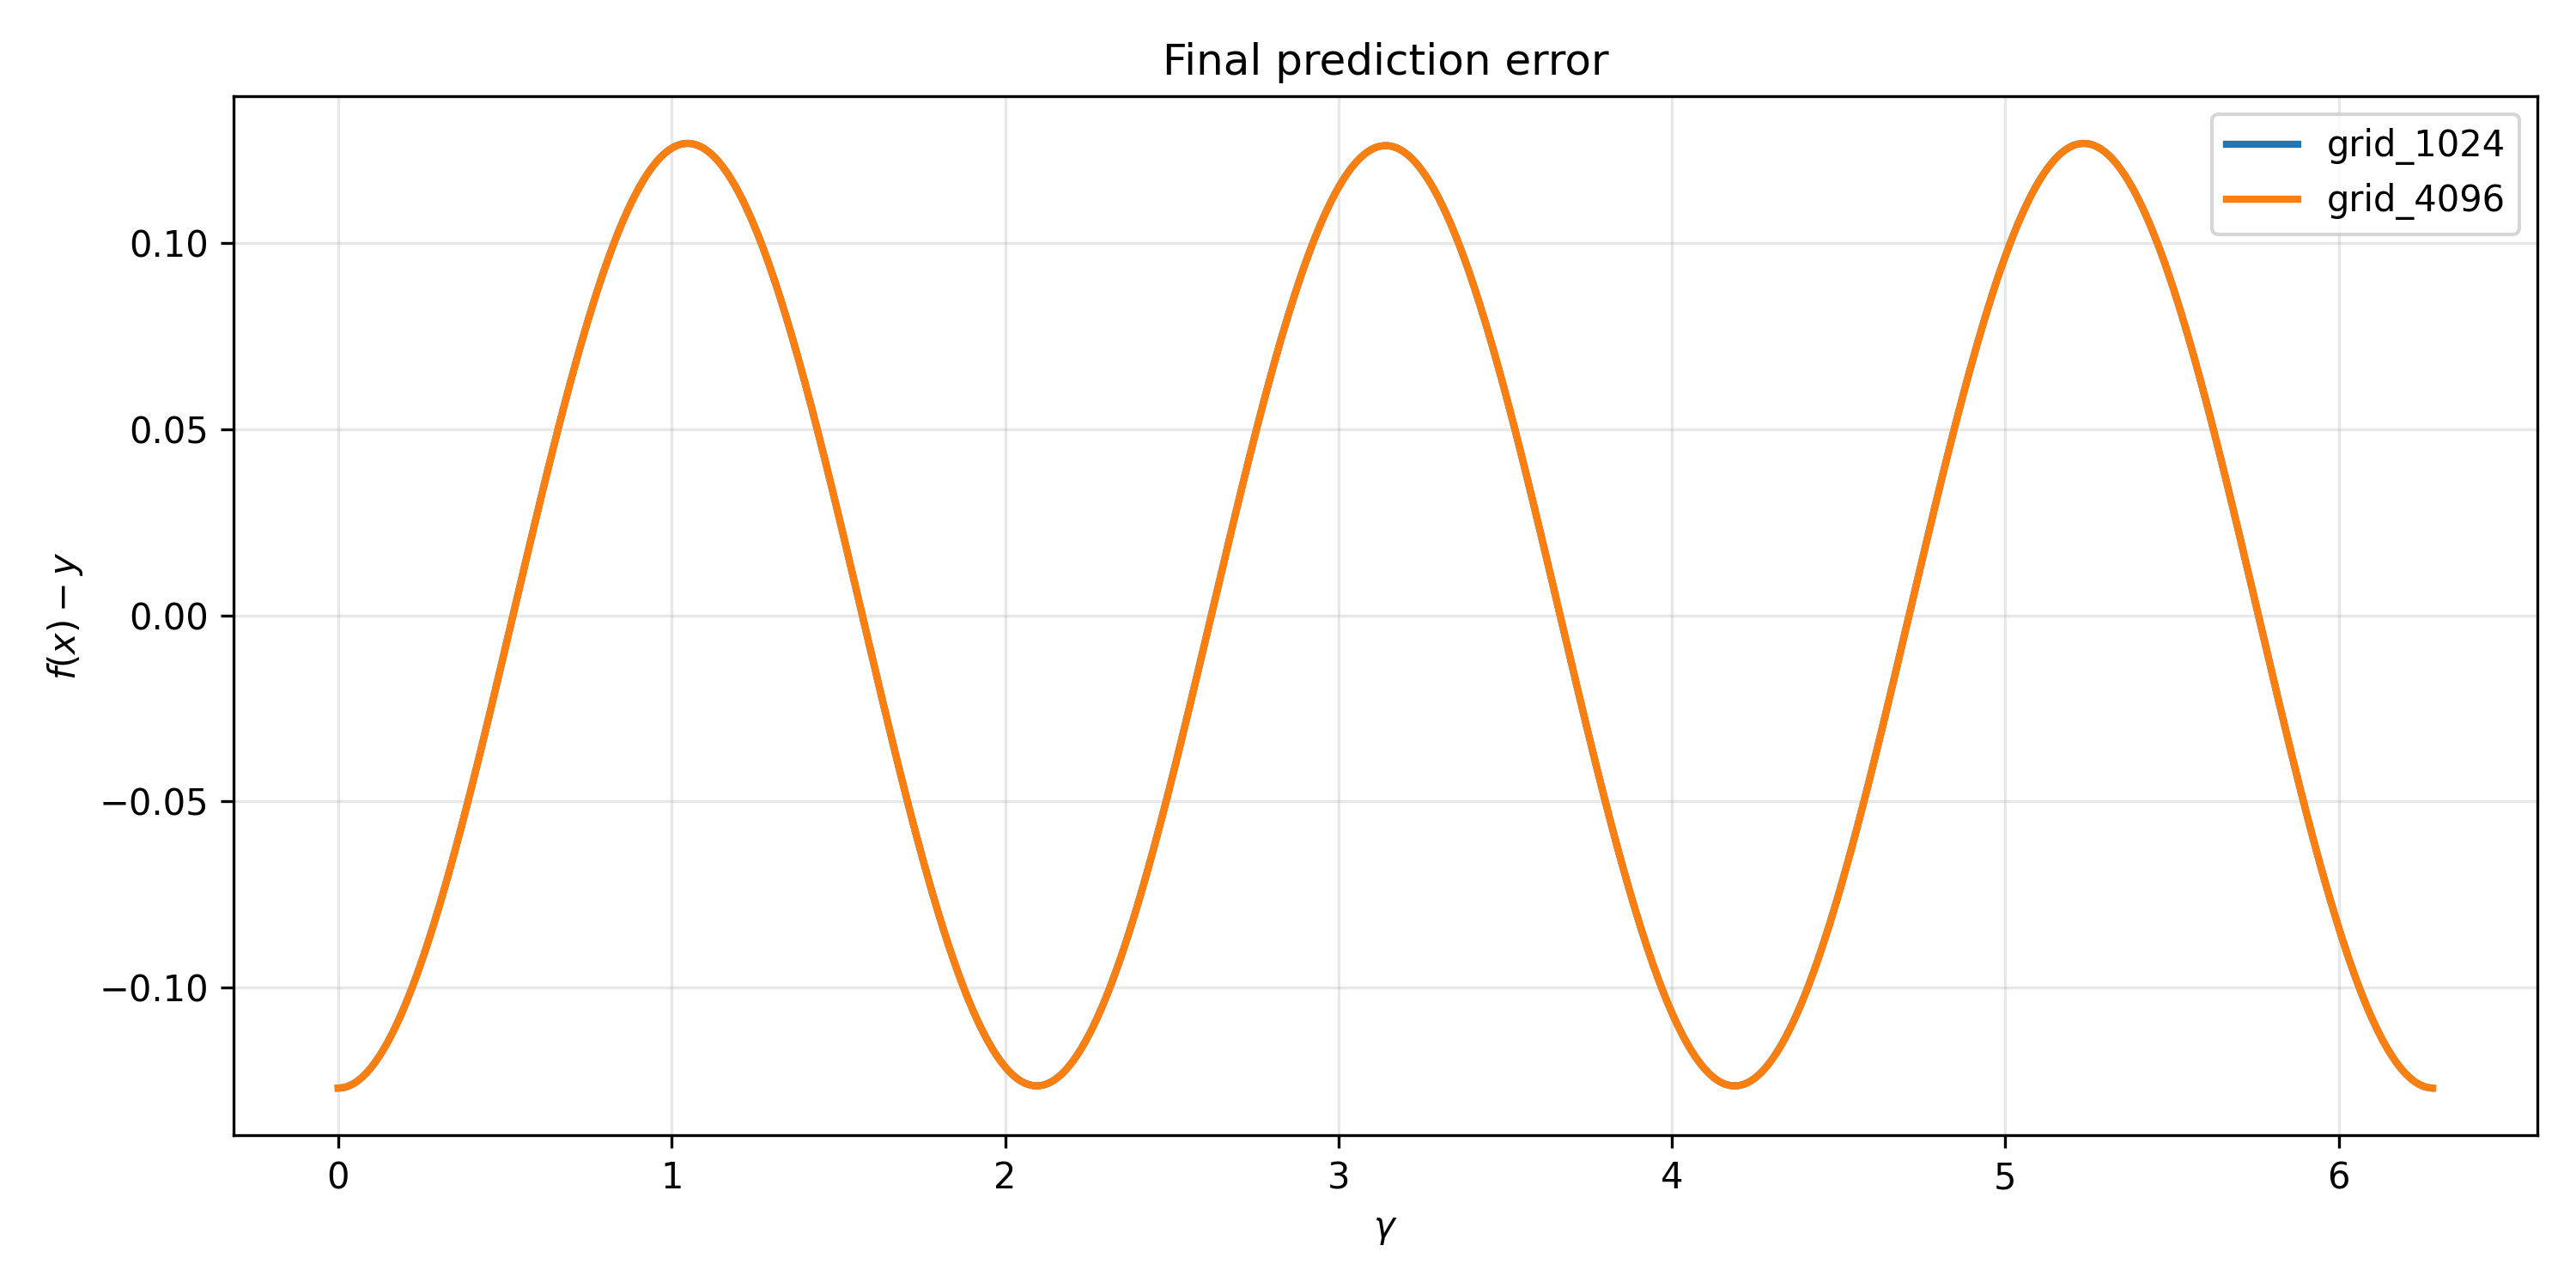
\includegraphics[width=\linewidth]{images/prediction_error_grid.png}
		\caption{Final prediction error}
	\end{subfigure}
	\caption{Additional plots for the grid-refinement experiment. The fitted functions and final errors for \texttt{grid\_1024} and \texttt{grid\_4096} remain nearly indistinguishable, consistent with the spectral comparison in the main text.}
\end{figure}

\begin{figure}[H]
	\centering
	\begin{subfigure}[t]{0.48\textwidth}
		\centering
		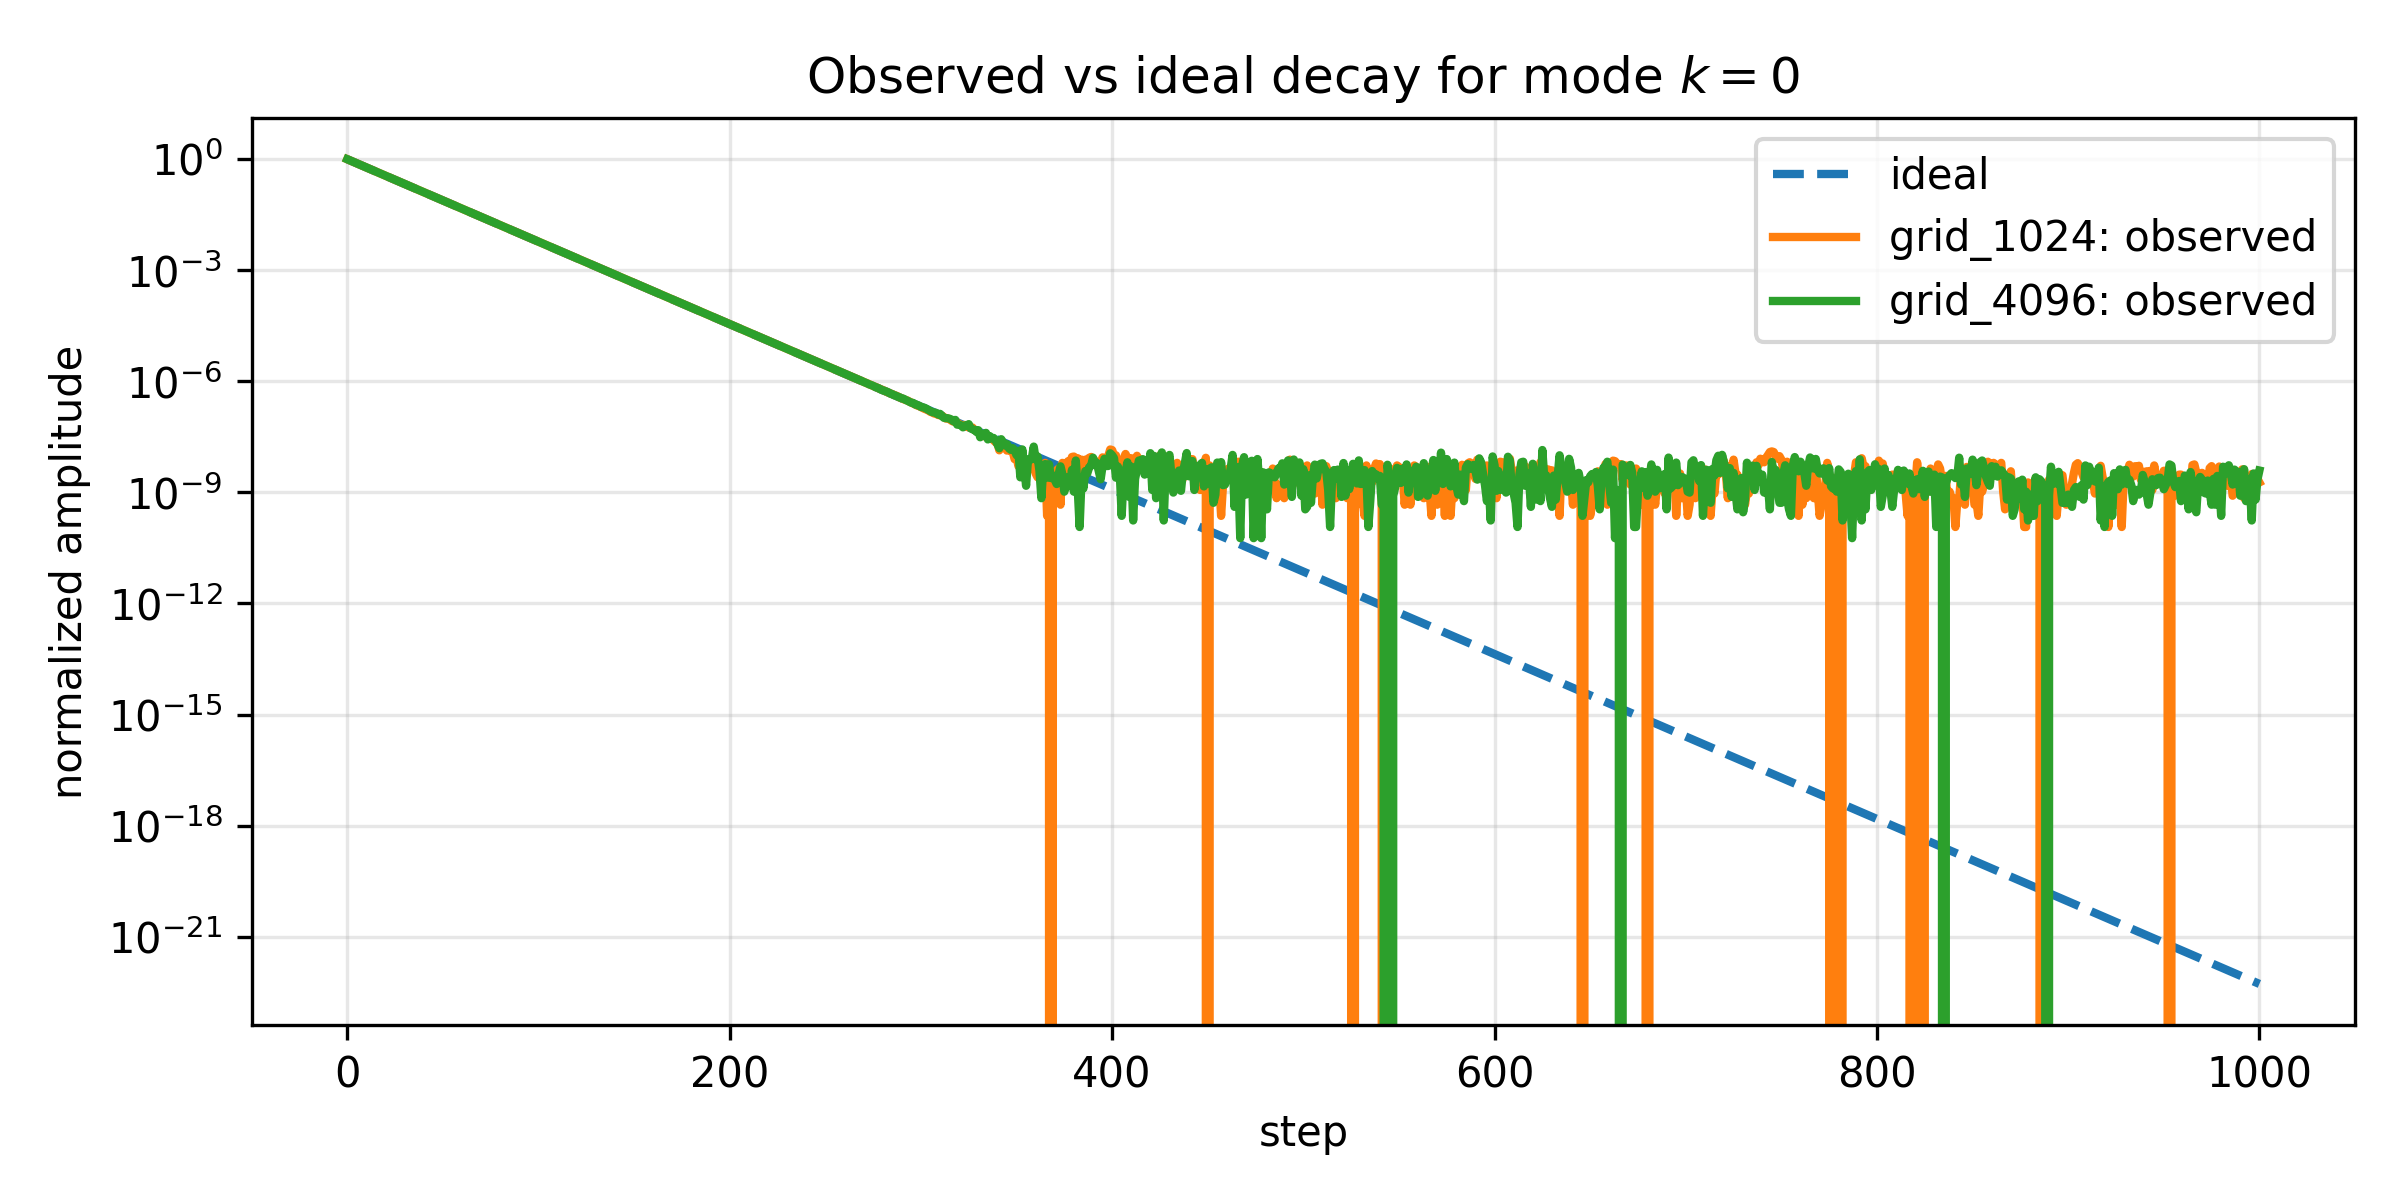
\includegraphics[width=\linewidth]{images/observed_vs_ideal_residual_decay_grid_mode_0.png}
		\caption{Mode $k=0$}
	\end{subfigure}
	\hfill
	\begin{subfigure}[t]{0.48\textwidth}
		\centering
		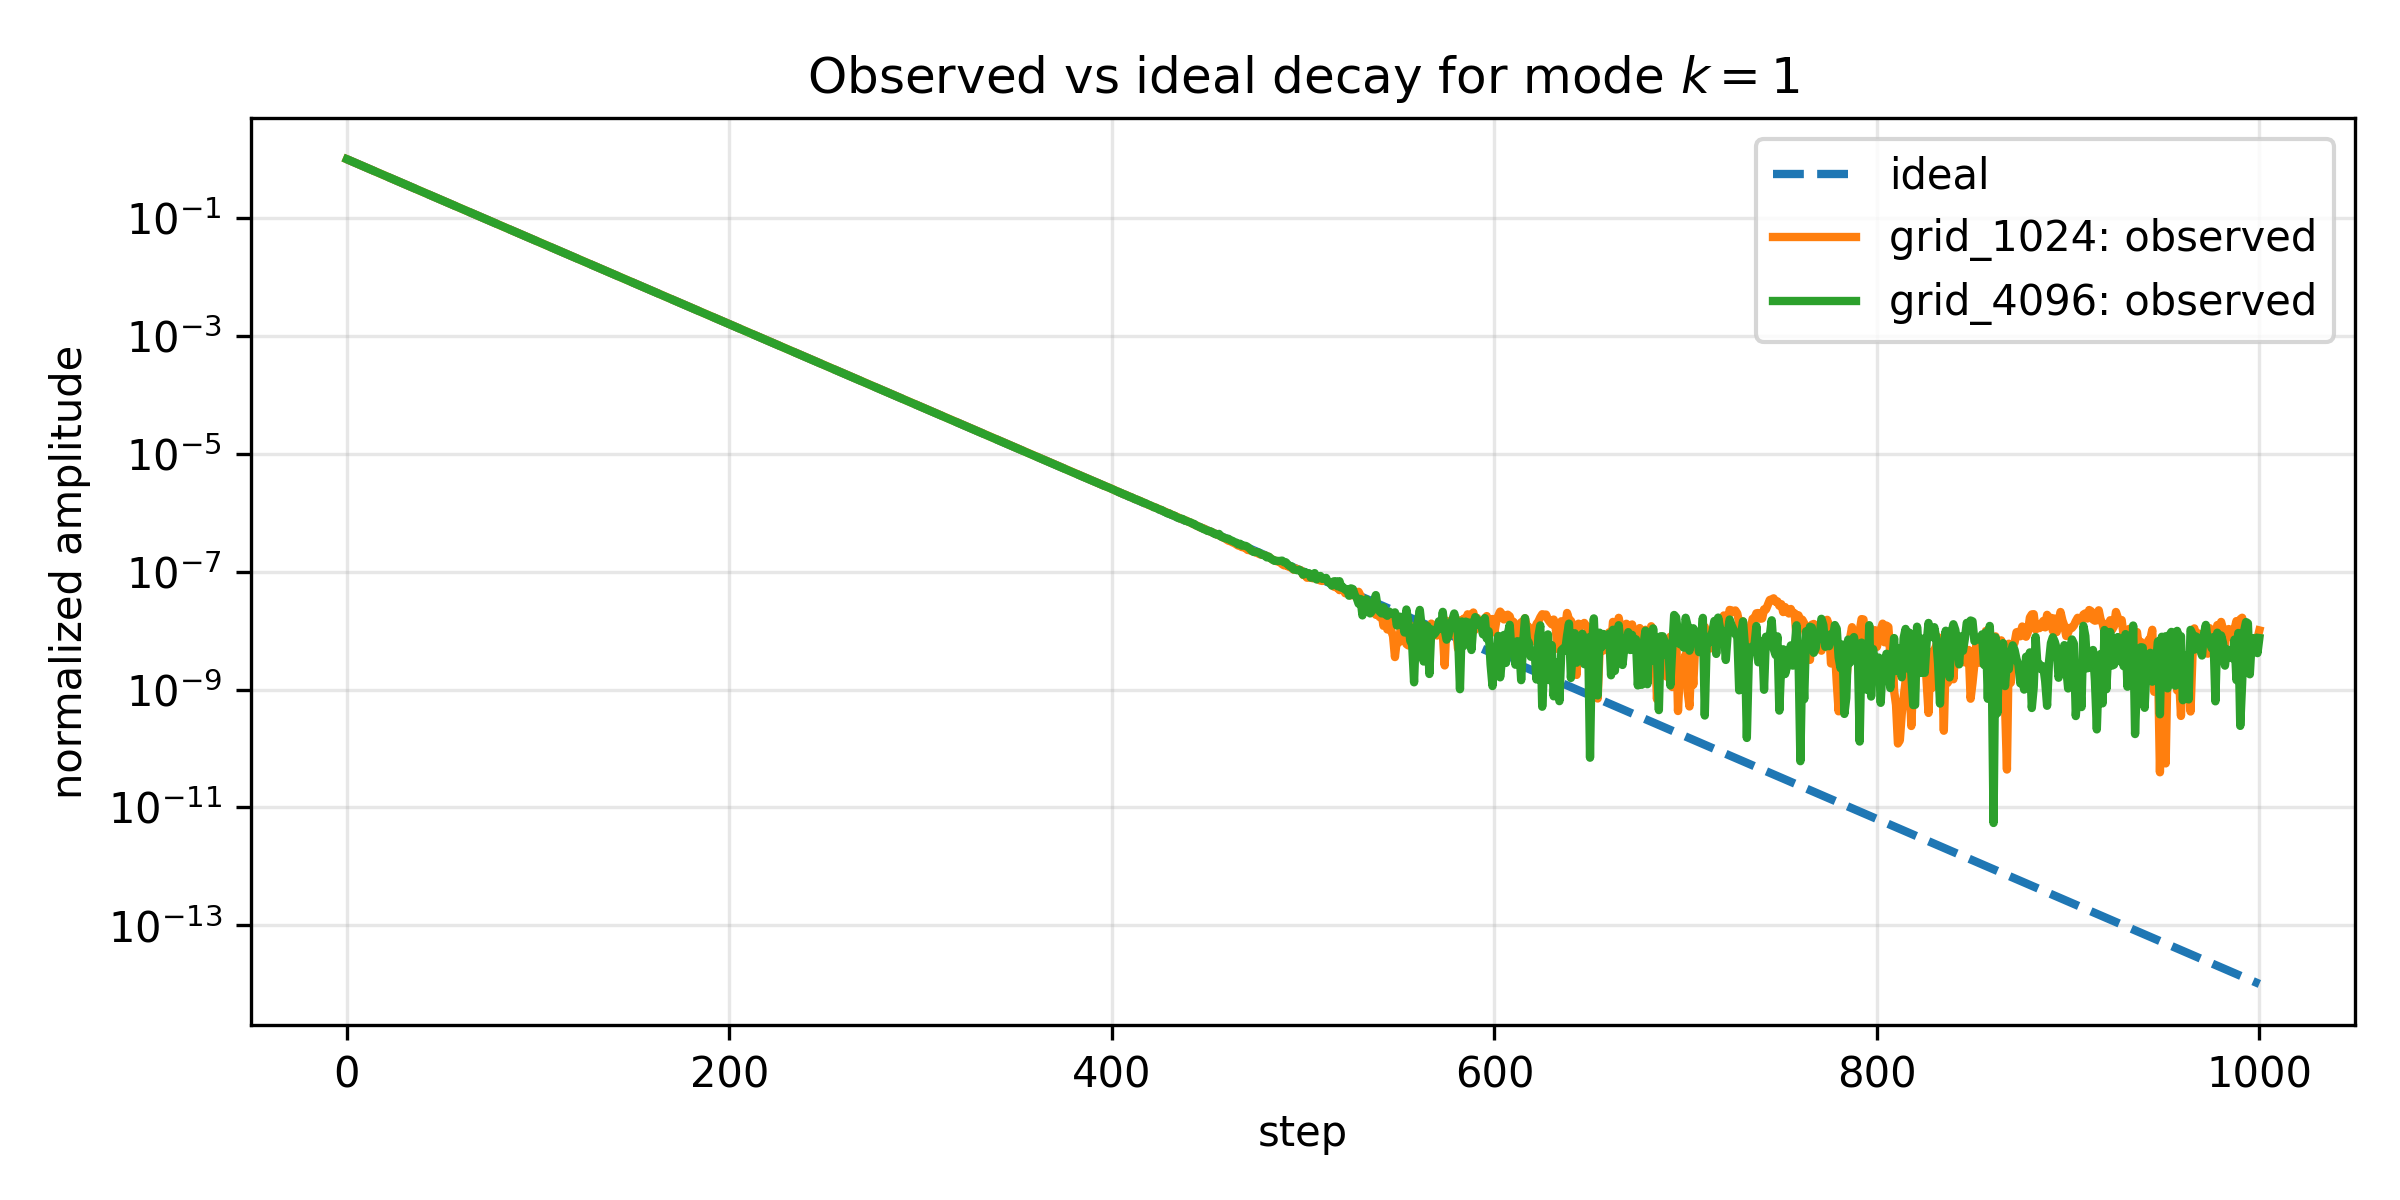
\includegraphics[width=\linewidth]{images/observed_vs_ideal_residual_decay_grid_mode_1.png}
		\caption{Mode $k=1$}
	\end{subfigure}

	\vspace{0.6em}

	\begin{subfigure}[t]{0.48\textwidth}
		\centering
		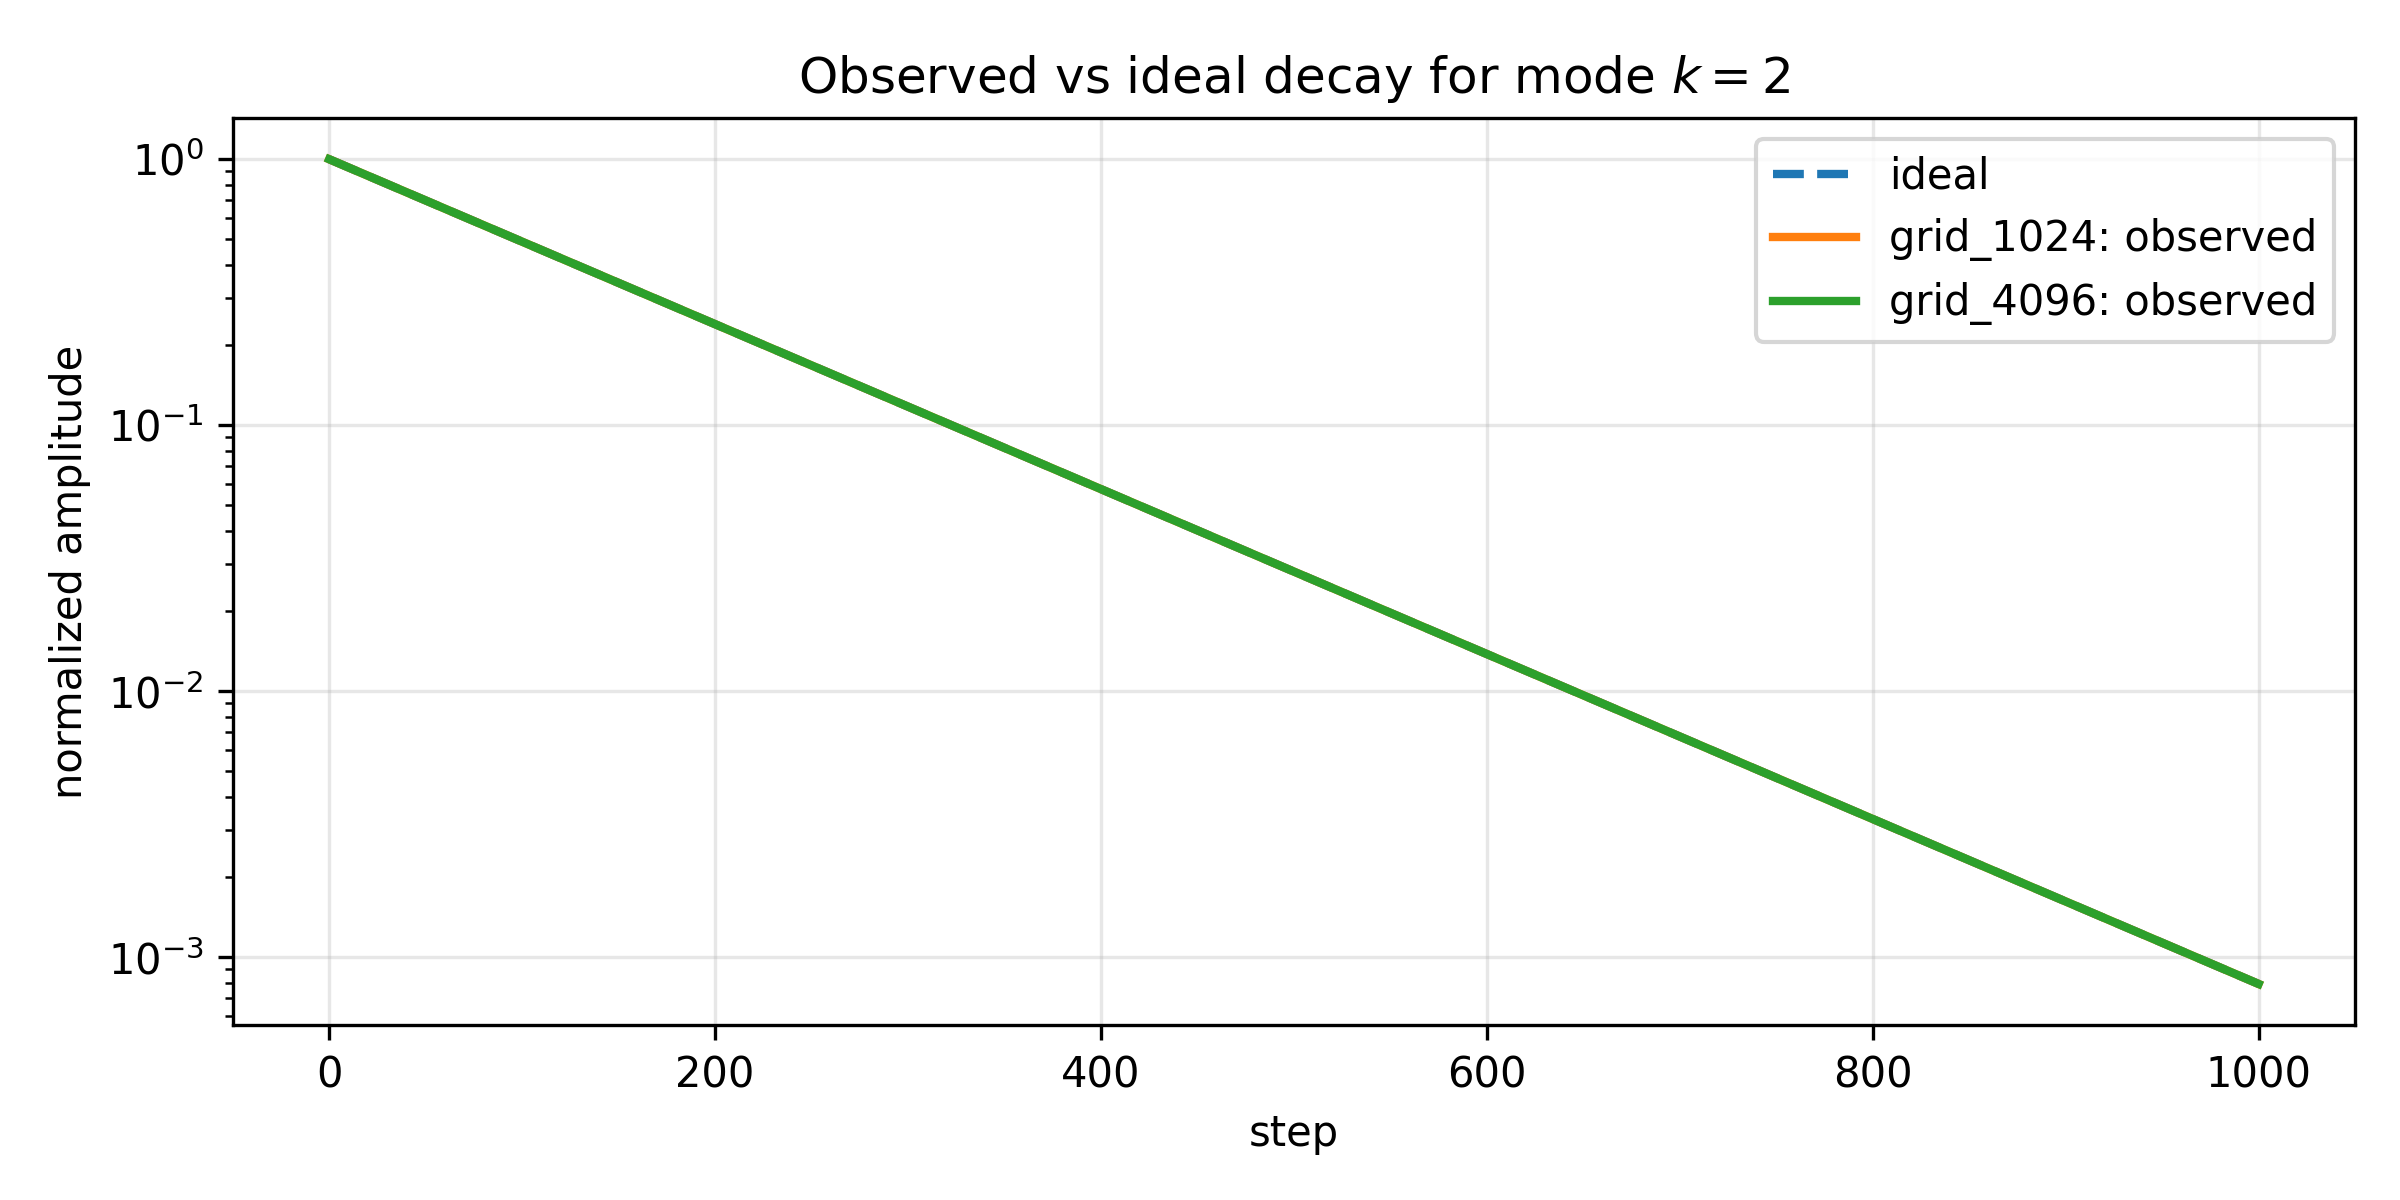
\includegraphics[width=\linewidth]{images/observed_vs_ideal_residual_decay_grid_mode_2.png}
		\caption{Mode $k=2$}
	\end{subfigure}
	\hfill
	\begin{subfigure}[t]{0.48\textwidth}
		\centering
		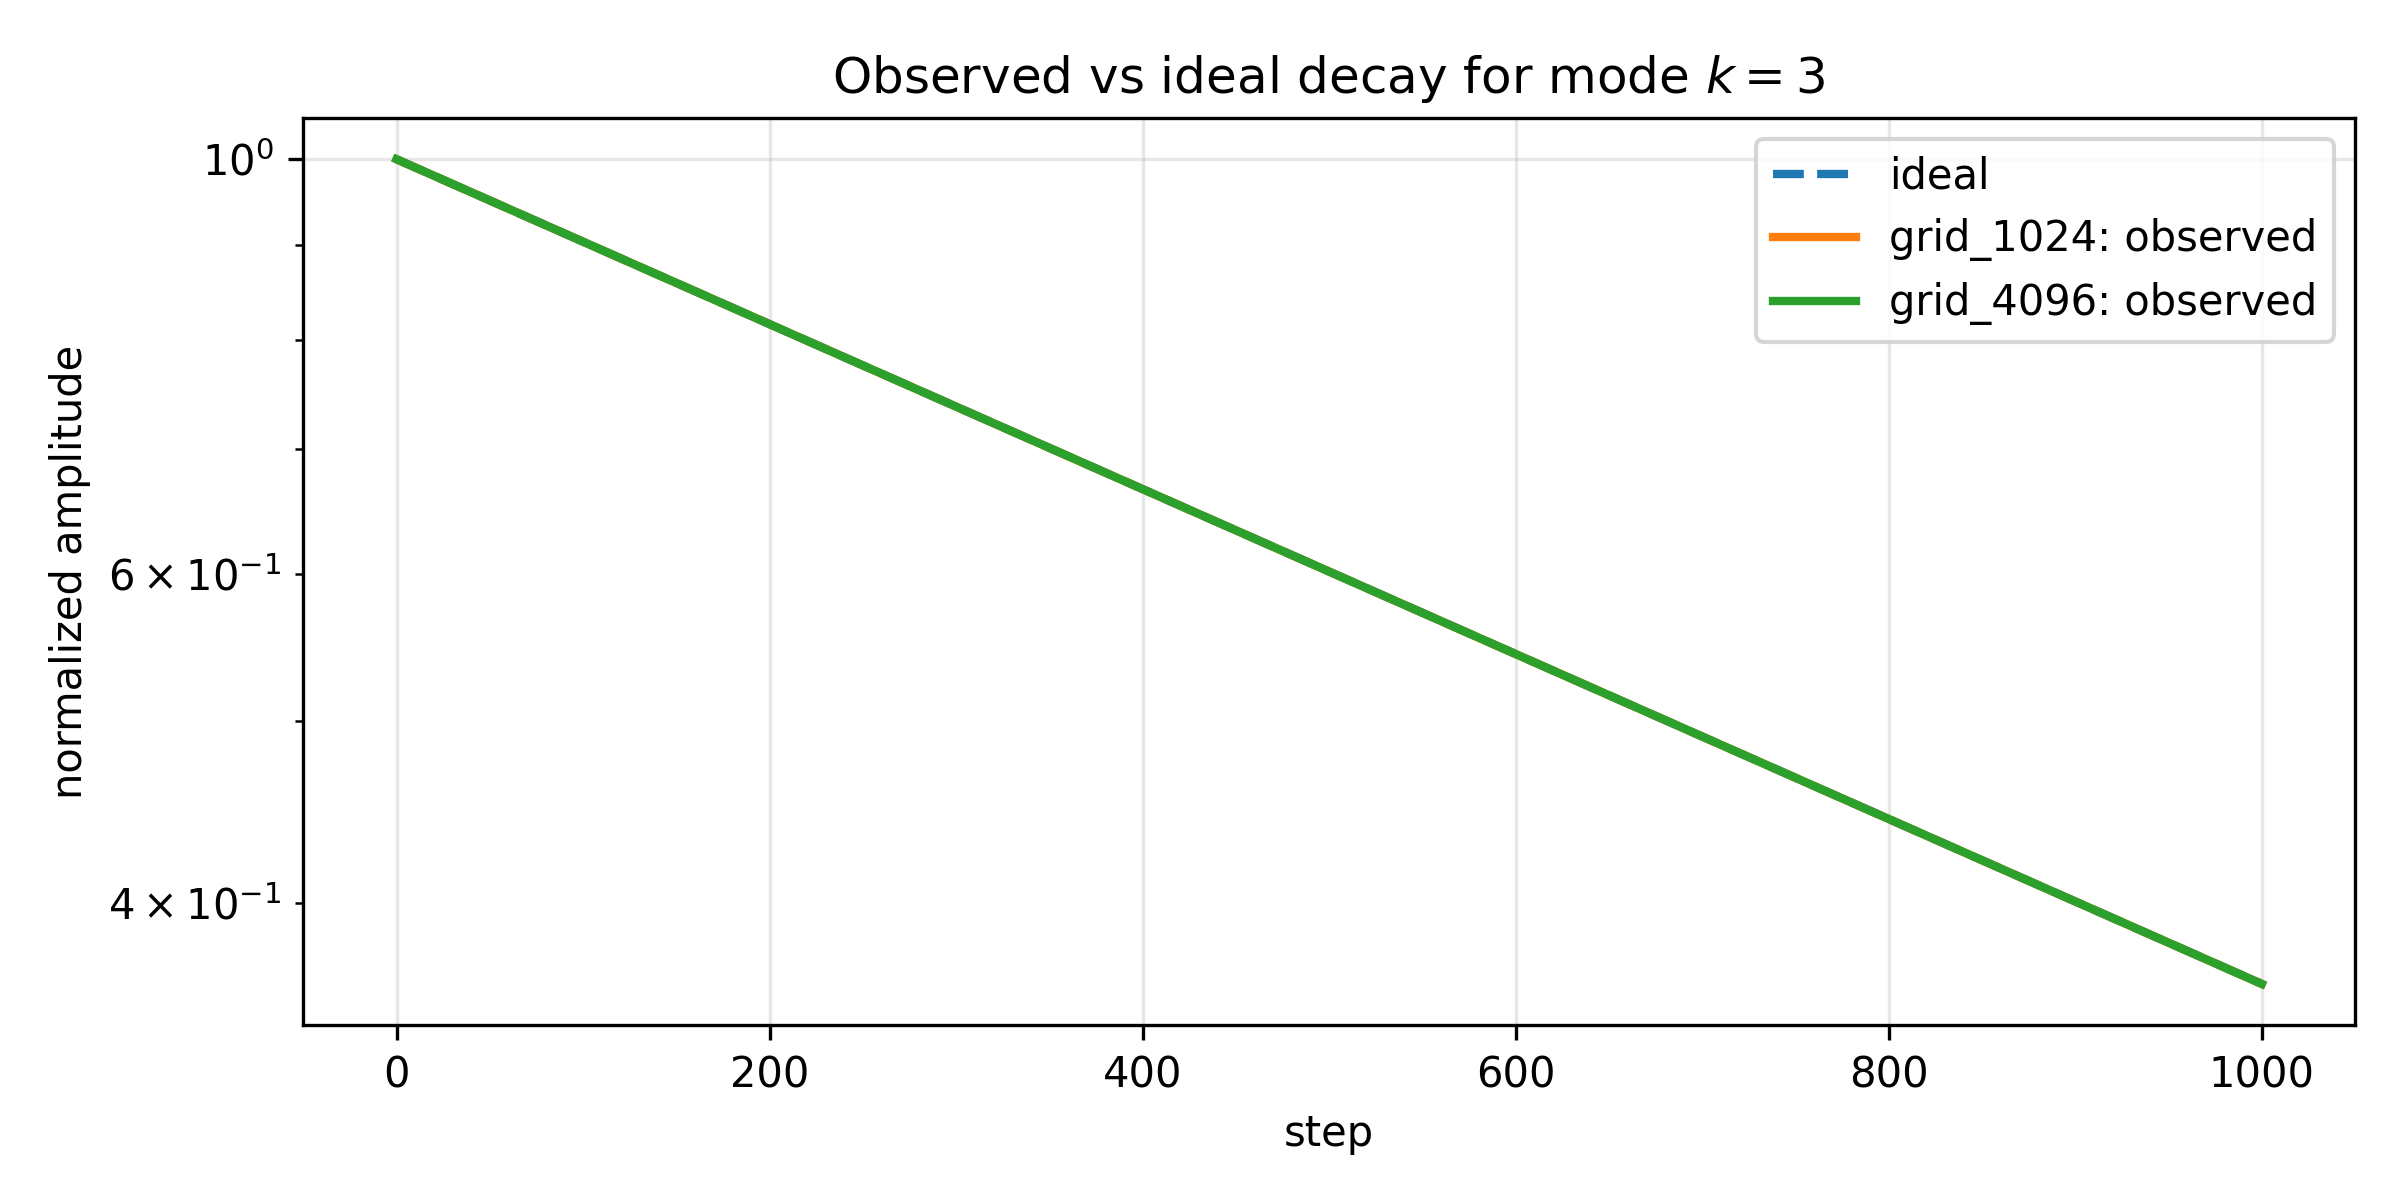
\includegraphics[width=\linewidth]{images/observed_vs_ideal_residual_decay_grid_mode_3.png}
		\caption{Mode $k=3$}
	\end{subfigure}
	\caption{Observed versus ideal normalized residual decay for the grid-refinement experiment. The two grid sizes behave almost identically across all active modes, with visible deviations only when the fastest modes reach the numerical floor.}
\end{figure}

\subsection*{B. Additional plots for the amplitude-swap experiment}

These plots support the distinction between normalized and unnormalized mode decay: the rate law is unchanged across targets, while the absolute residual remains larger when more initial mass is placed in slower modes.

\begin{figure}[H]
	\centering
	\begin{subfigure}[t]{0.48\textwidth}
		\centering
		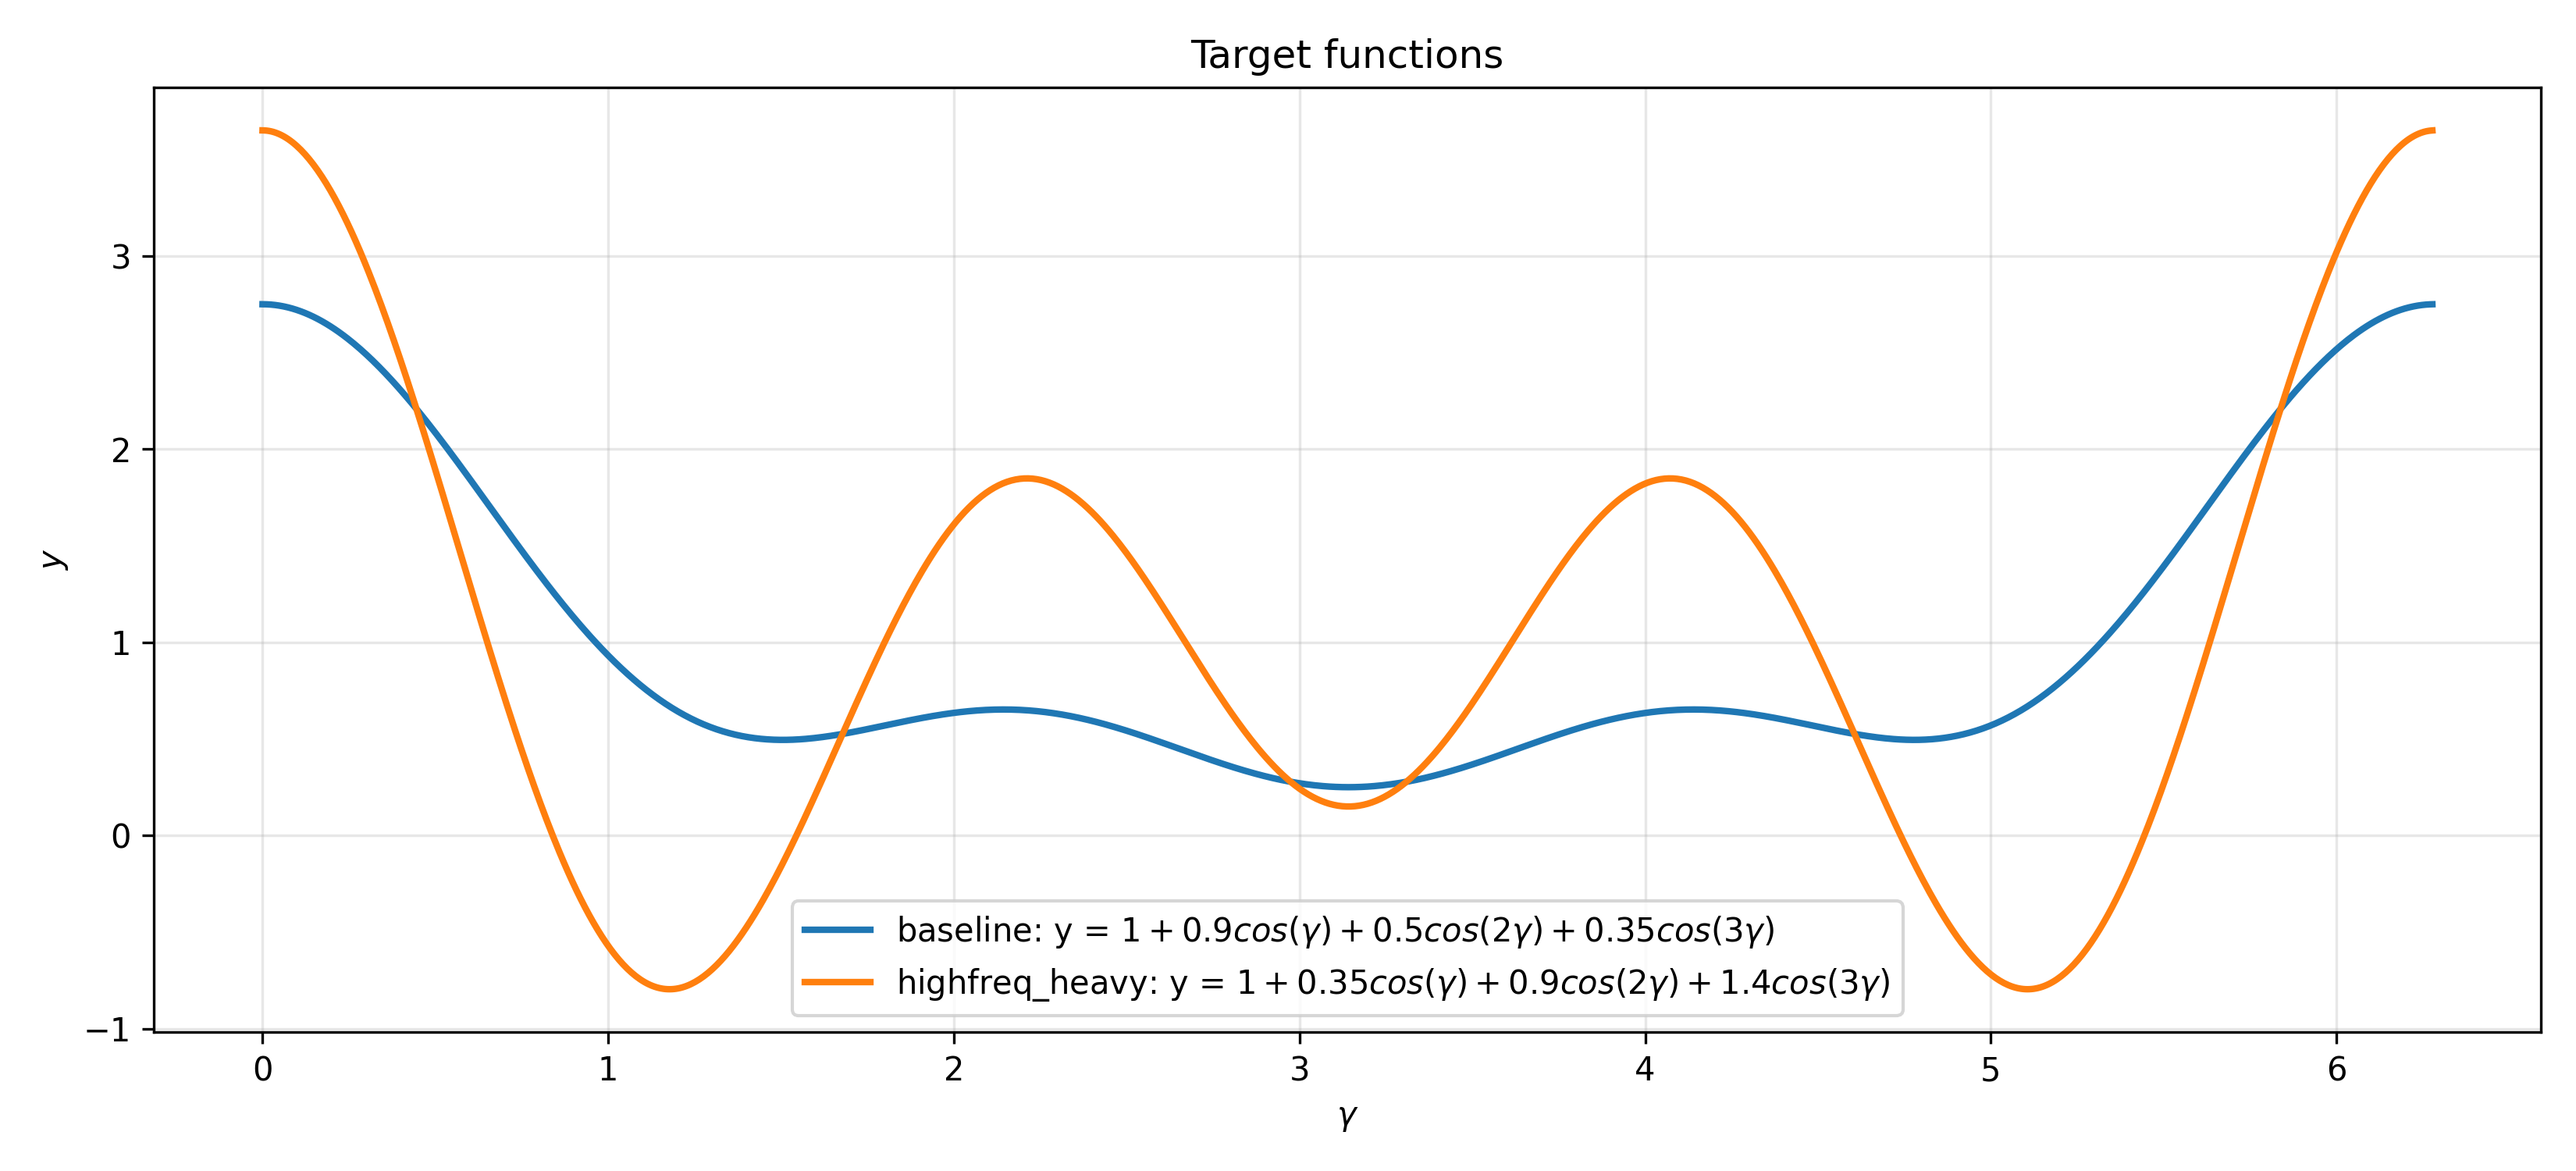
\includegraphics[width=\linewidth]{images/target_functions.png}
		\caption{Target functions}
	\end{subfigure}
	\hfill
	\begin{subfigure}[t]{0.48\textwidth}
		\centering
		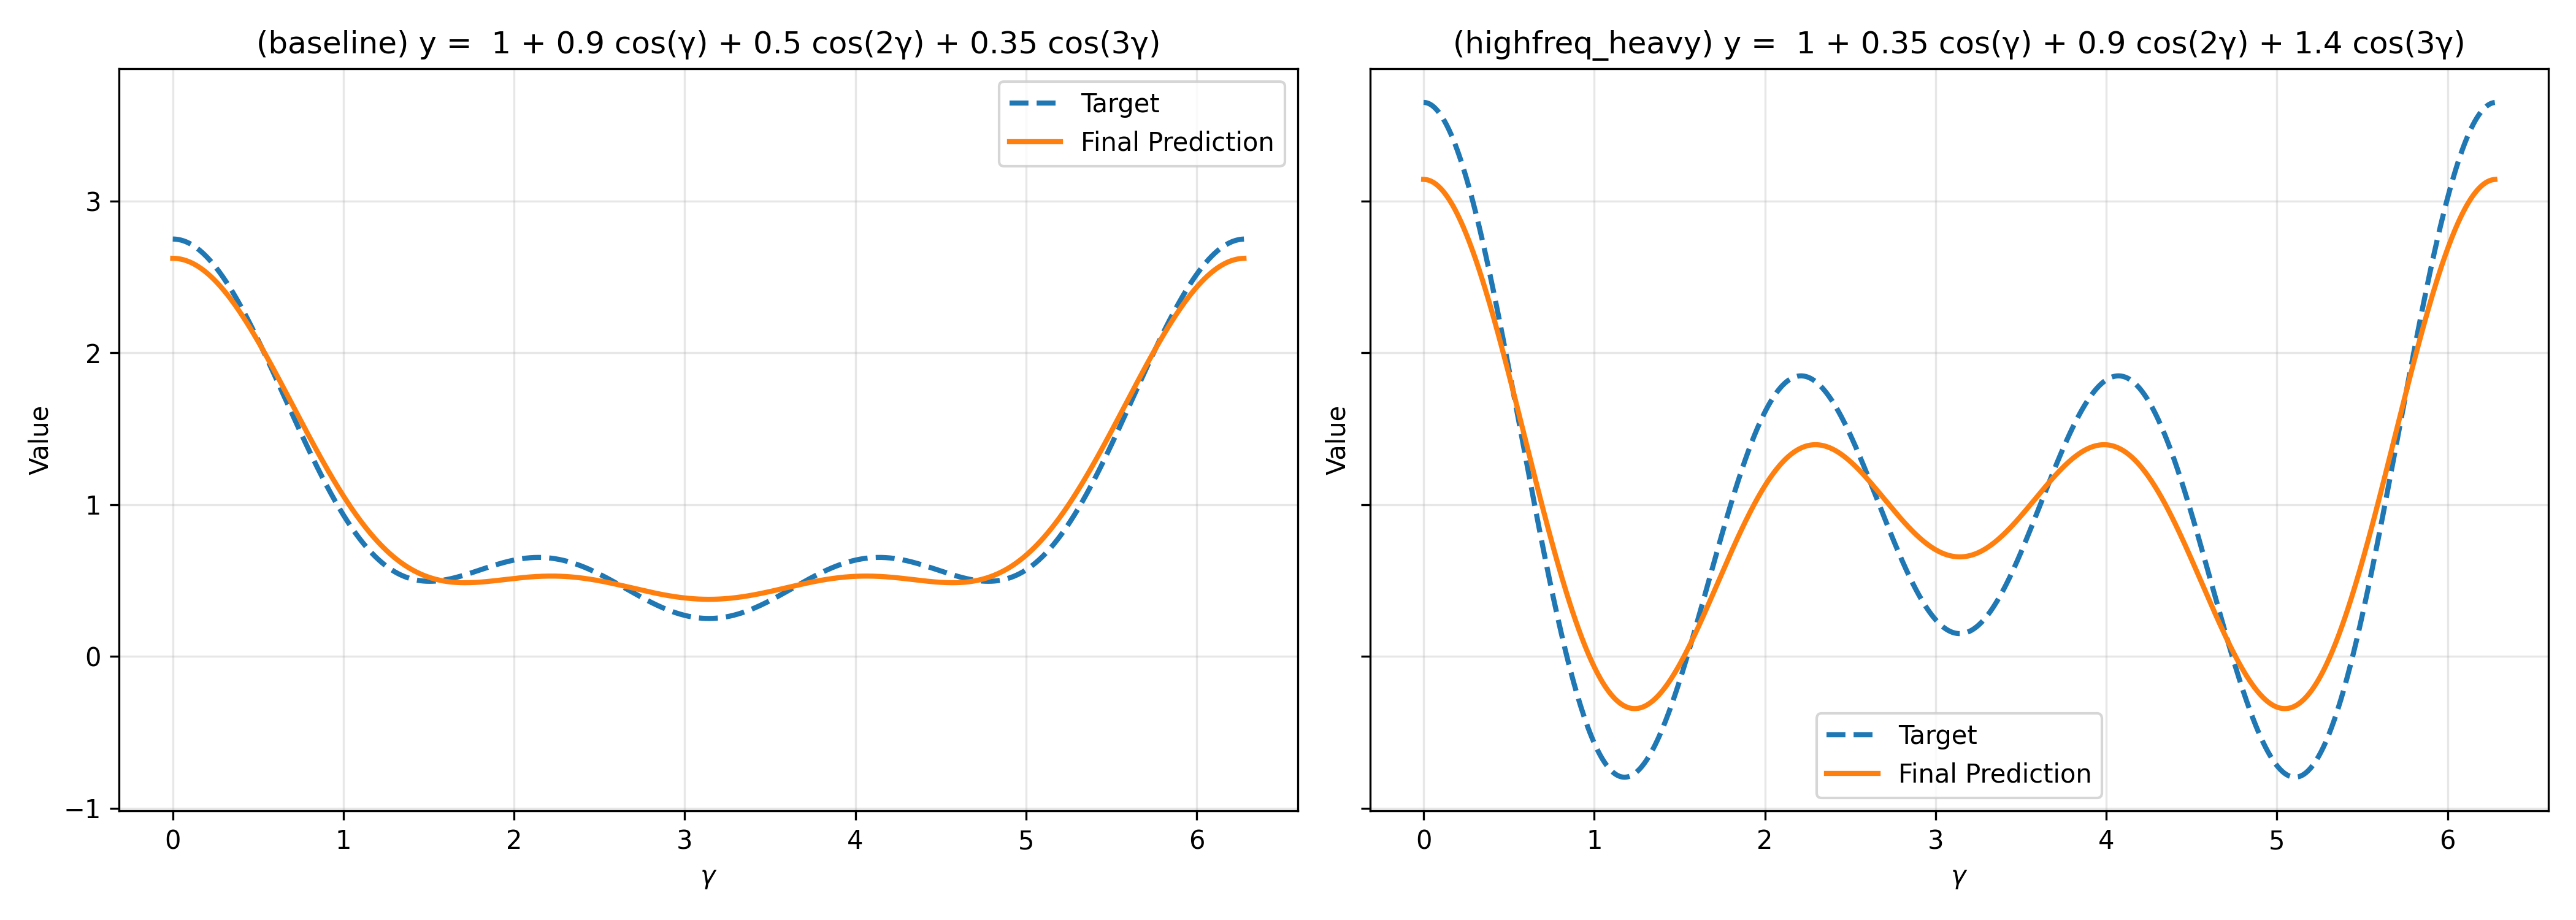
\includegraphics[width=\linewidth]{images/final_predictions_baseline_vs_highfreq.png}
		\caption{Final predictions}
	\end{subfigure}
	\caption{Baseline versus high-frequency-heavy target. The high-frequency-heavy target contains more mass in slow modes and is therefore fitted less well at the same training horizon.}
\end{figure}

\begin{figure}[H]
	\centering
	\begin{subfigure}[t]{0.48\textwidth}
		\centering
		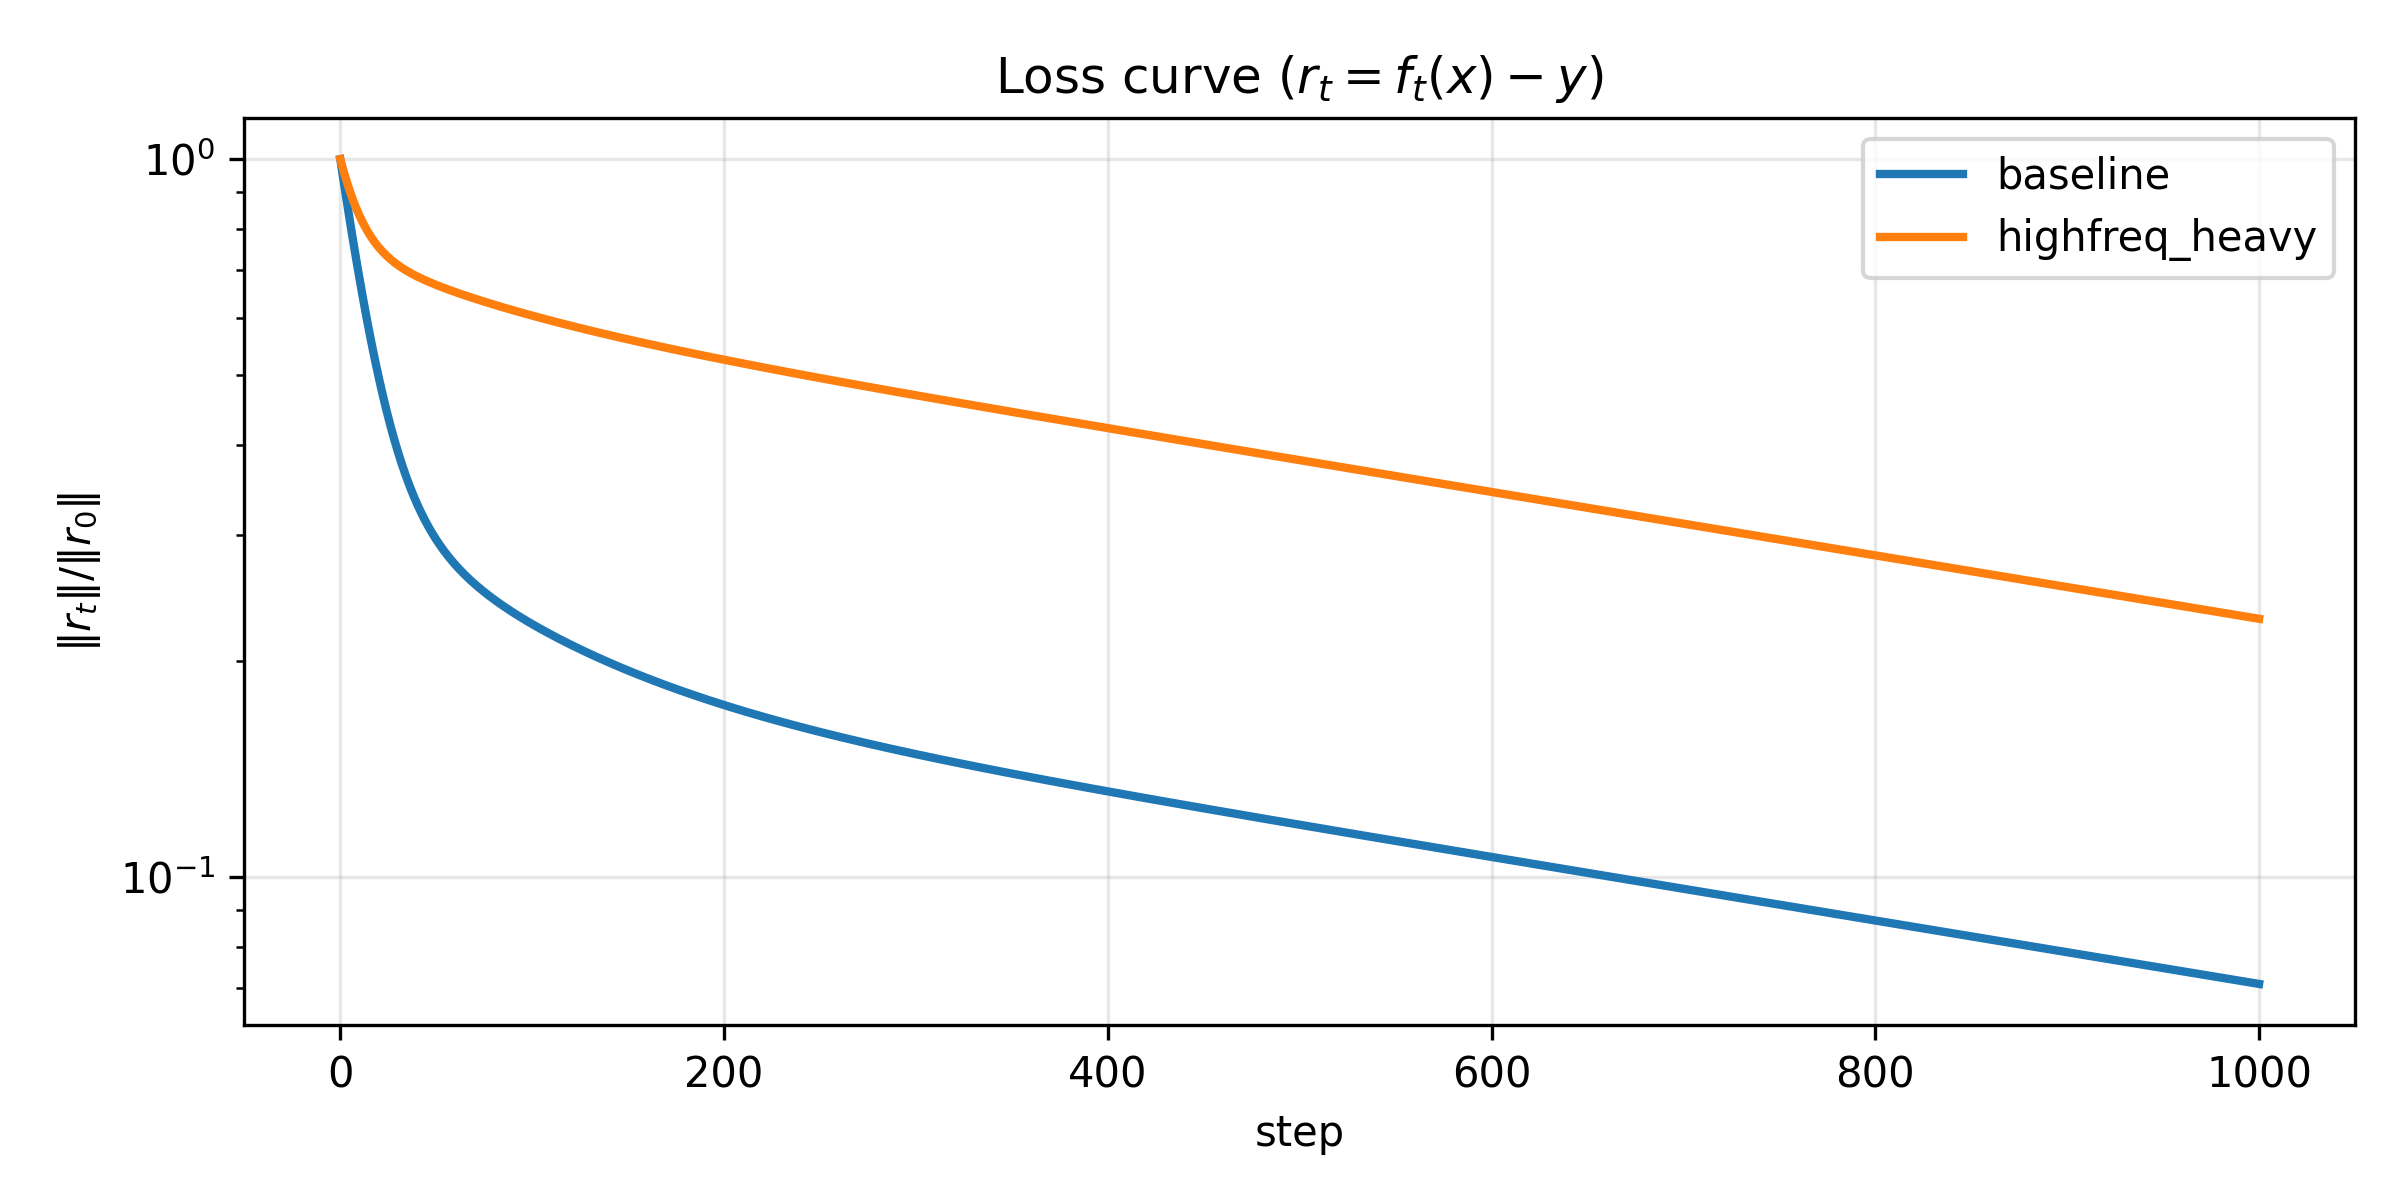
\includegraphics[width=\linewidth]{images/loss_curve_baseline_vs_highfreq.png}
		\caption{Relative residual decay}
	\end{subfigure}
	\hfill
	\begin{subfigure}[t]{0.48\textwidth}
		\centering
		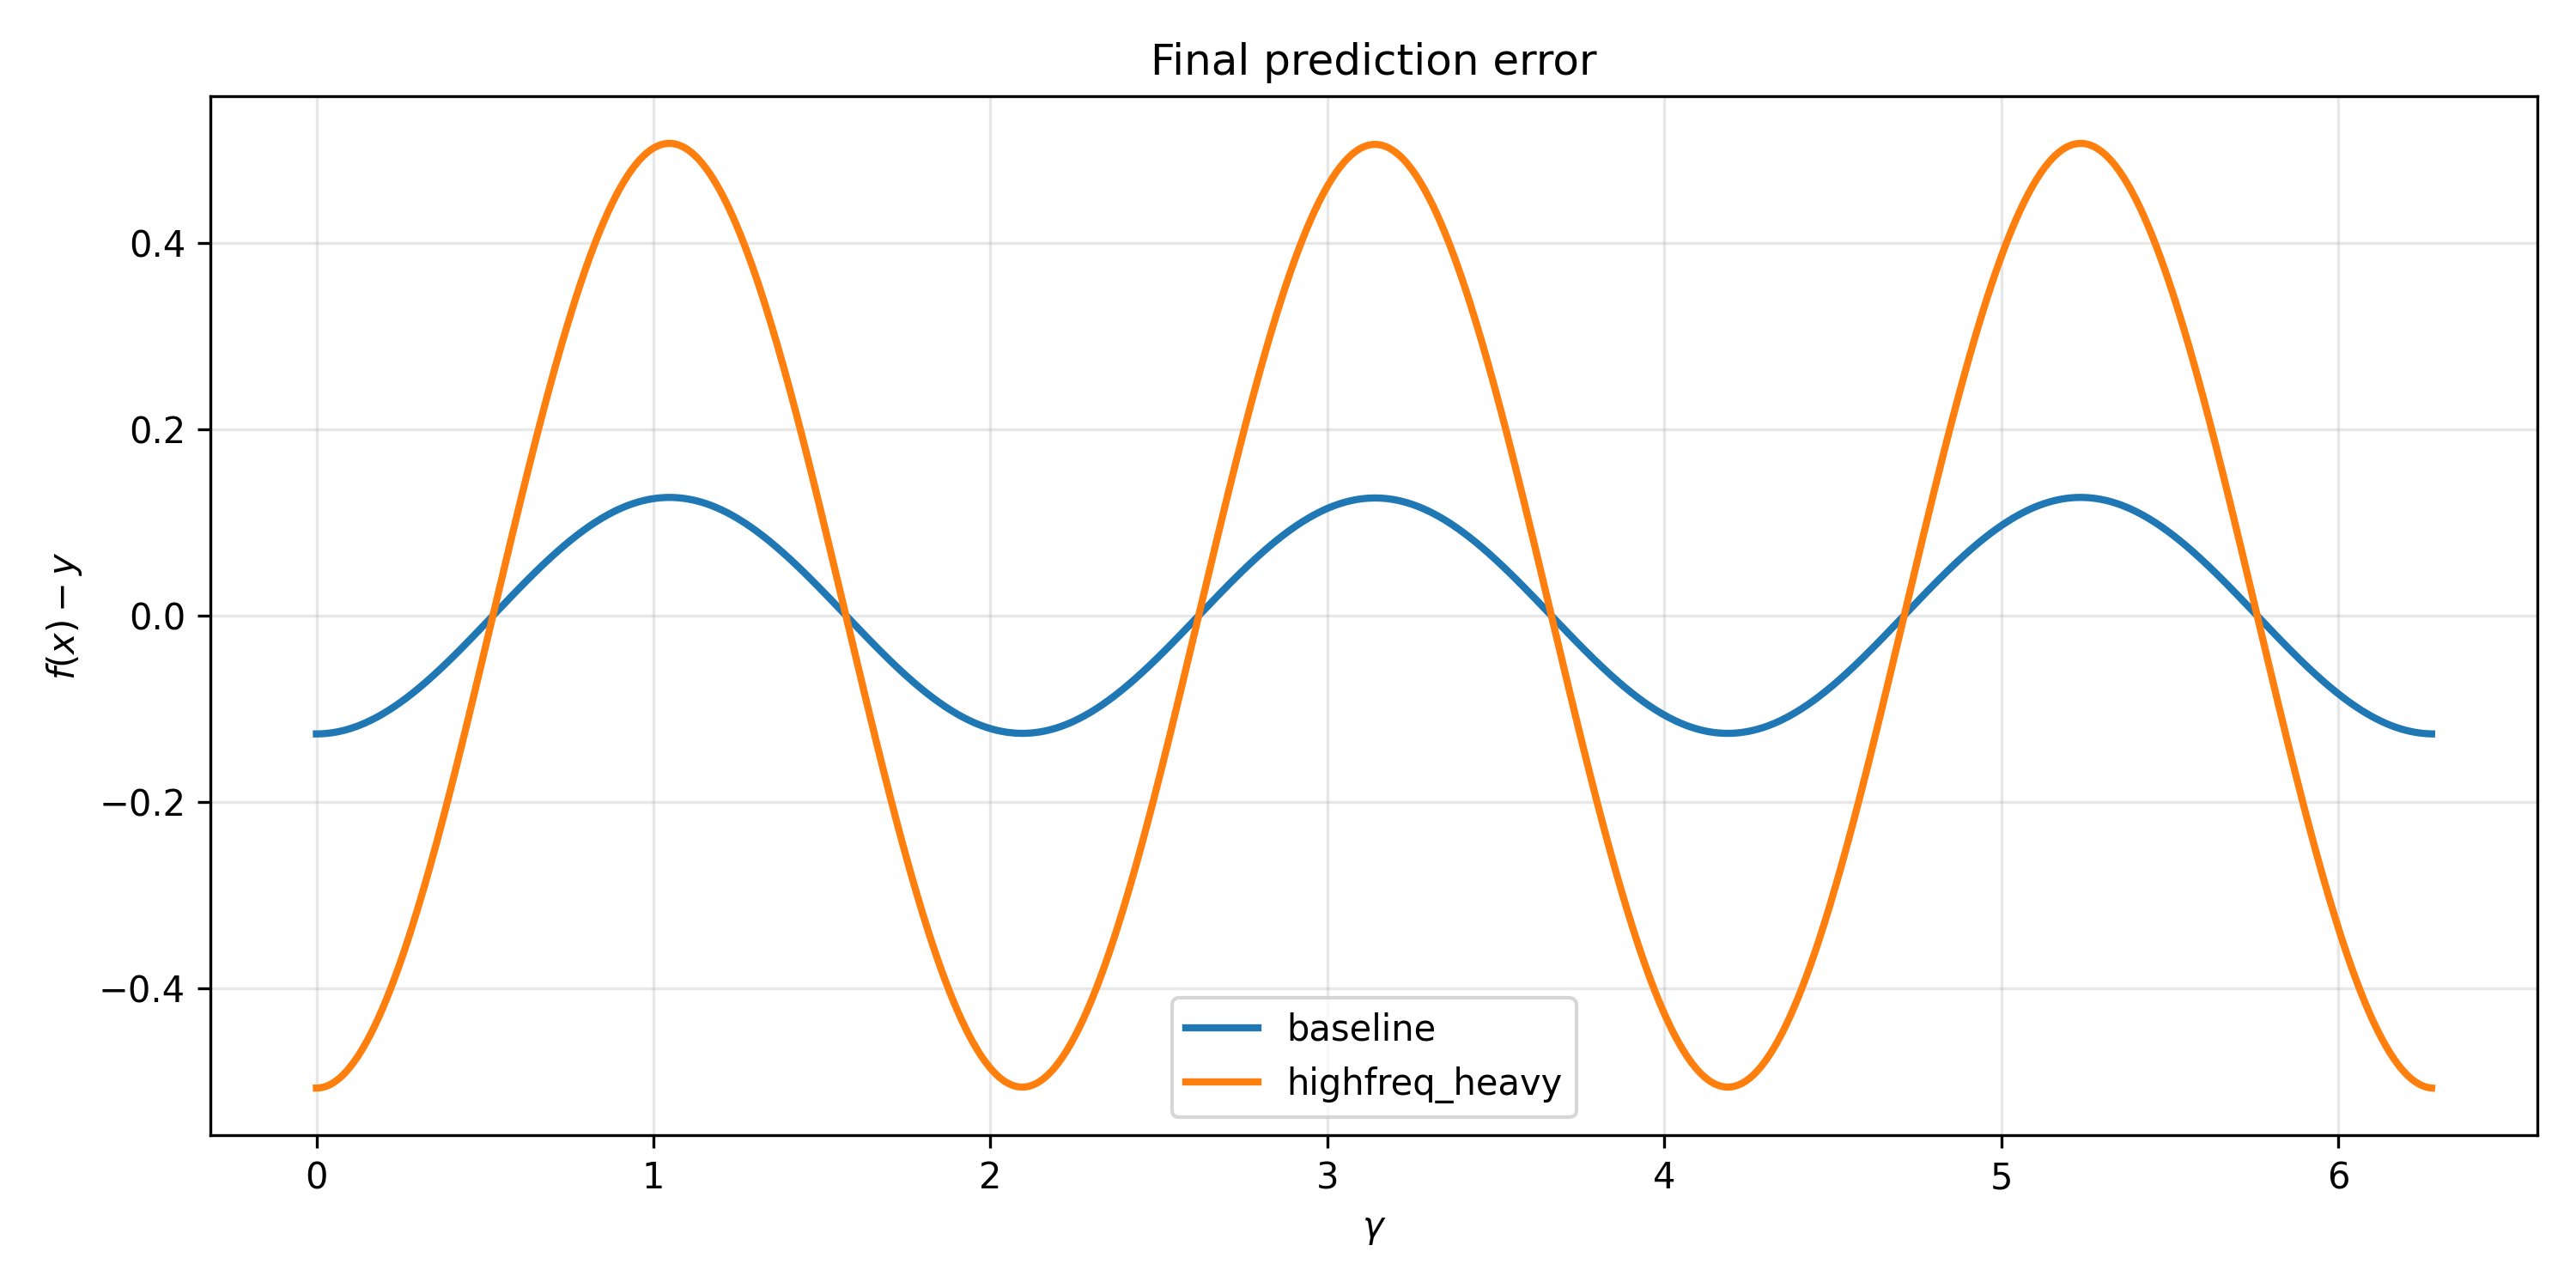
\includegraphics[width=\linewidth]{images/prediction_error_high_frequency.png}
		\caption{Final prediction error}
	\end{subfigure}
	\caption{Additional global diagnostics for the amplitude-swap experiment. The high-frequency-heavy target decays more slowly in overall residual norm and leaves a larger structured final error.}
\end{figure}

\begin{figure}[H]
	\centering
	\begin{subfigure}[t]{0.48\textwidth}
		\centering
		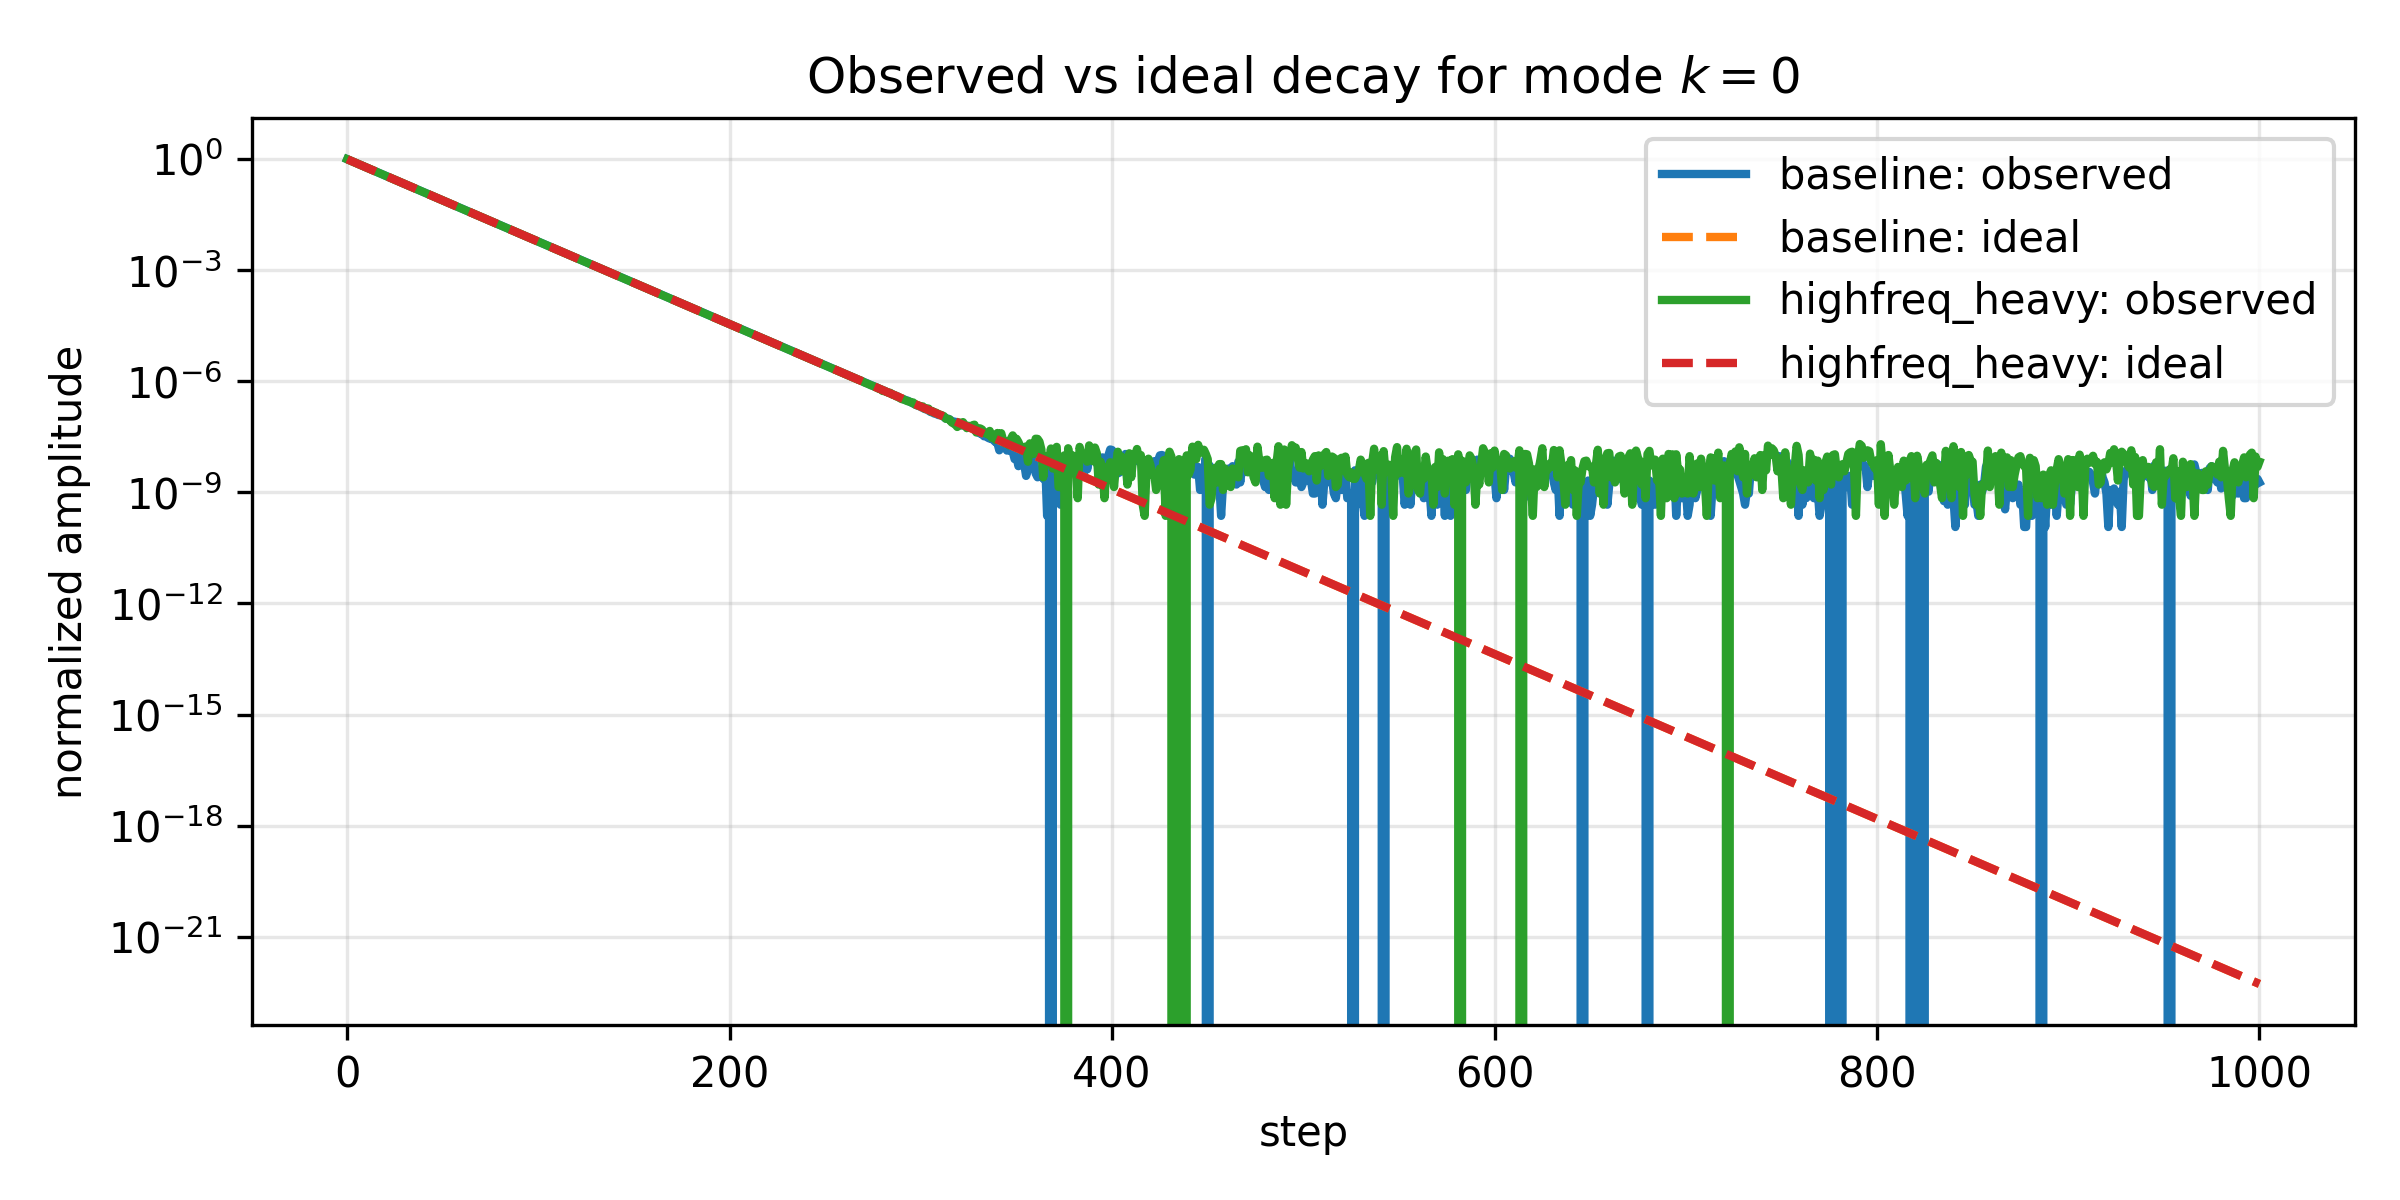
\includegraphics[width=\linewidth]{images/observed_vs_ideal_residual_decay_mode_0.png}
		\caption{Mode $k=0$}
	\end{subfigure}
	\hfill
	\begin{subfigure}[t]{0.48\textwidth}
		\centering
		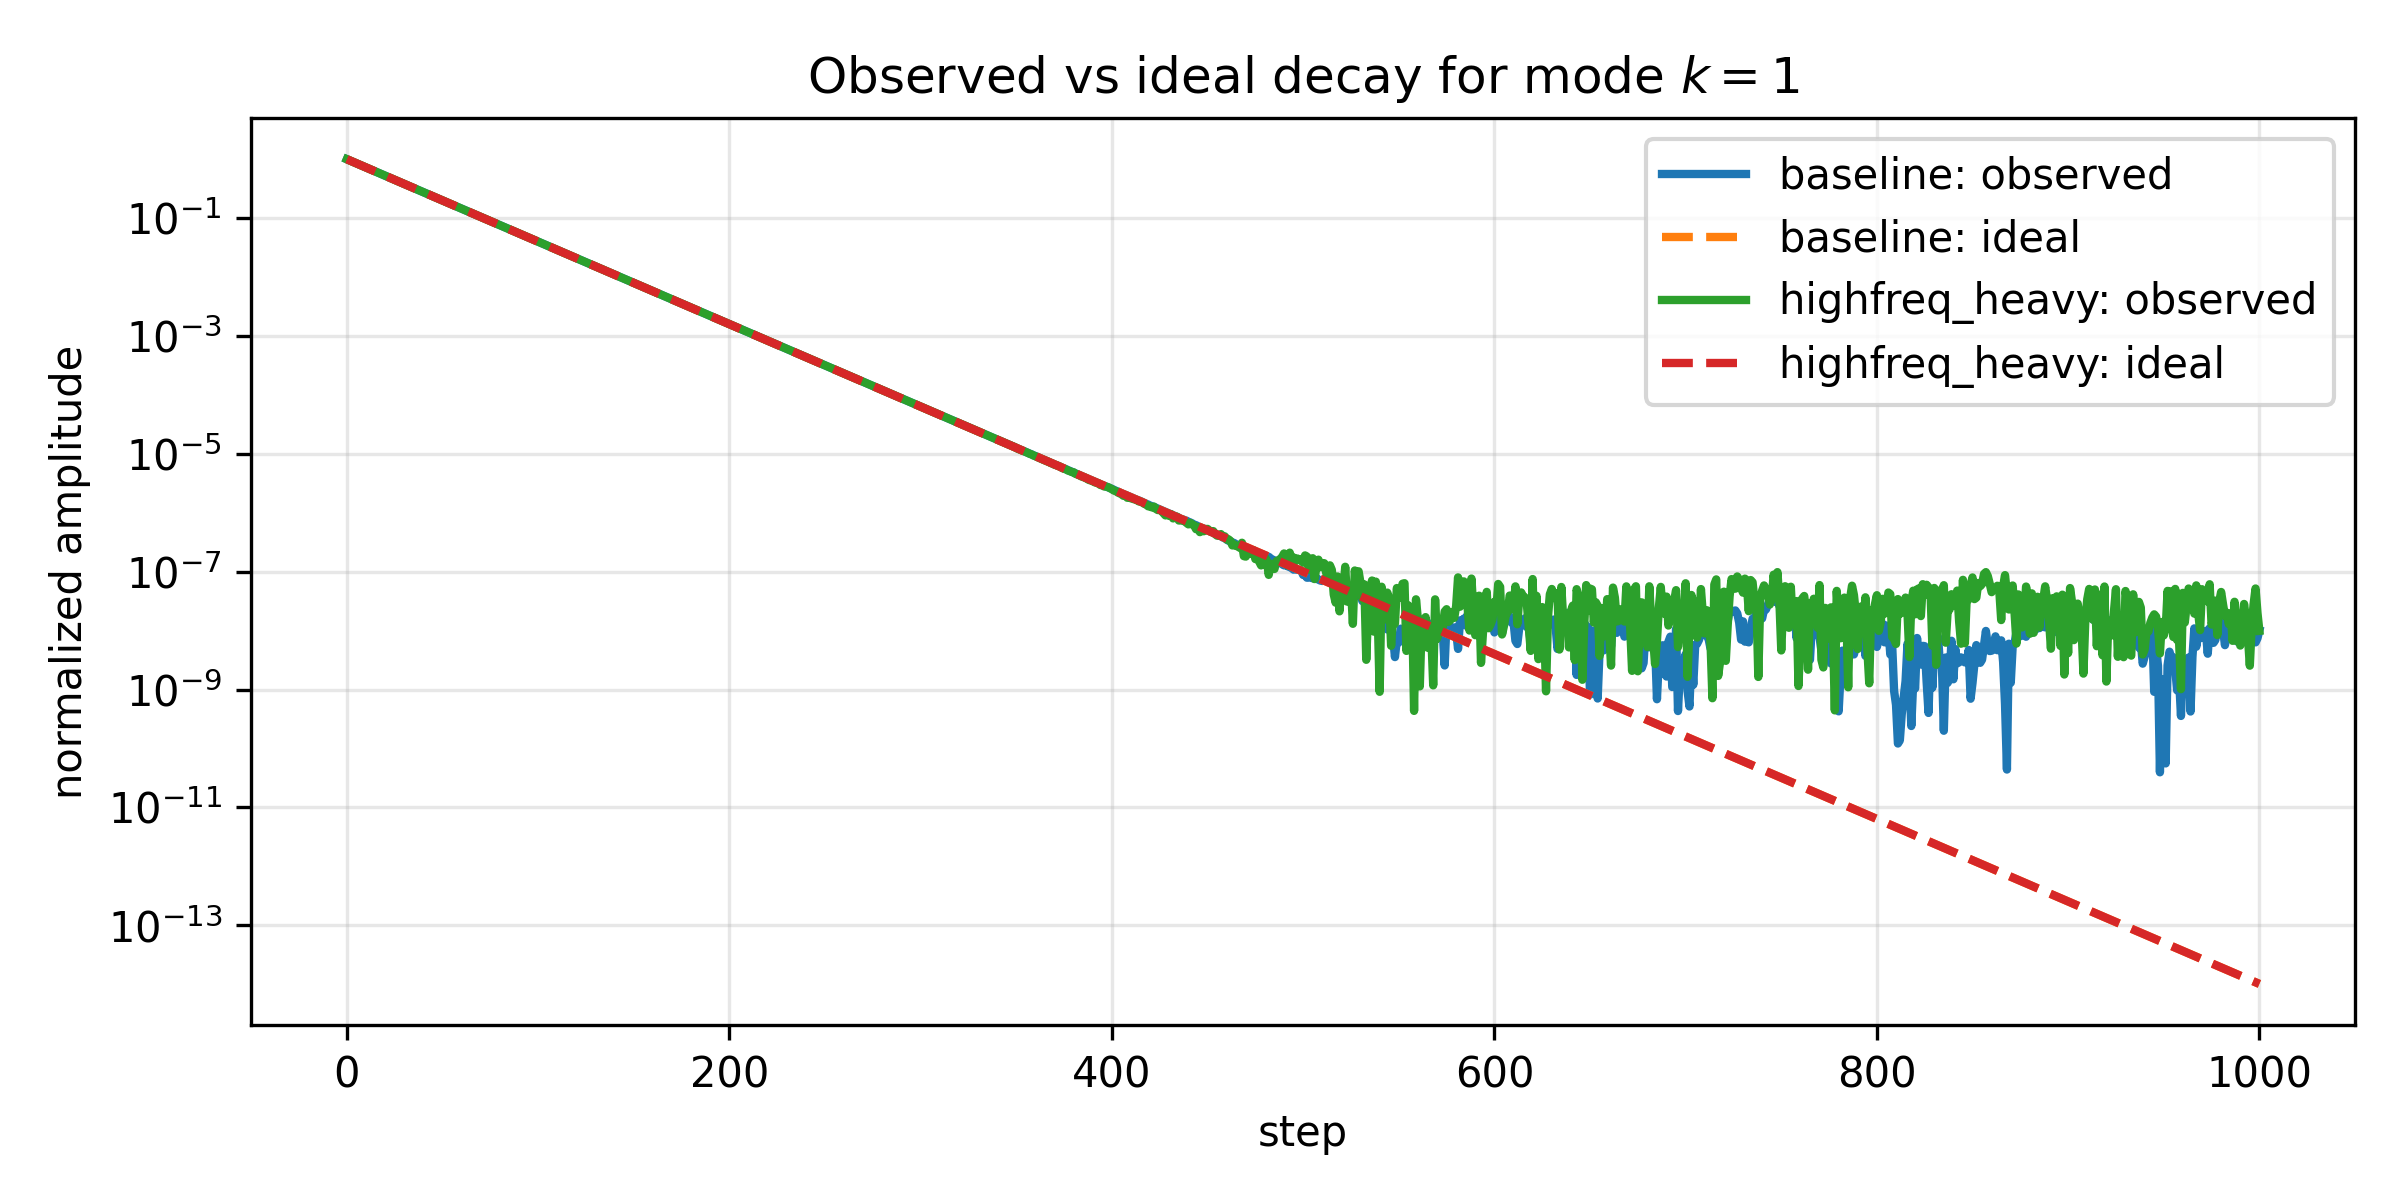
\includegraphics[width=\linewidth]{images/observed_vs_ideal_residual_decay_mode_1.png}
		\caption{Mode $k=1$}
	\end{subfigure}

	\vspace{0.6em}

	\begin{subfigure}[t]{0.48\textwidth}
		\centering
		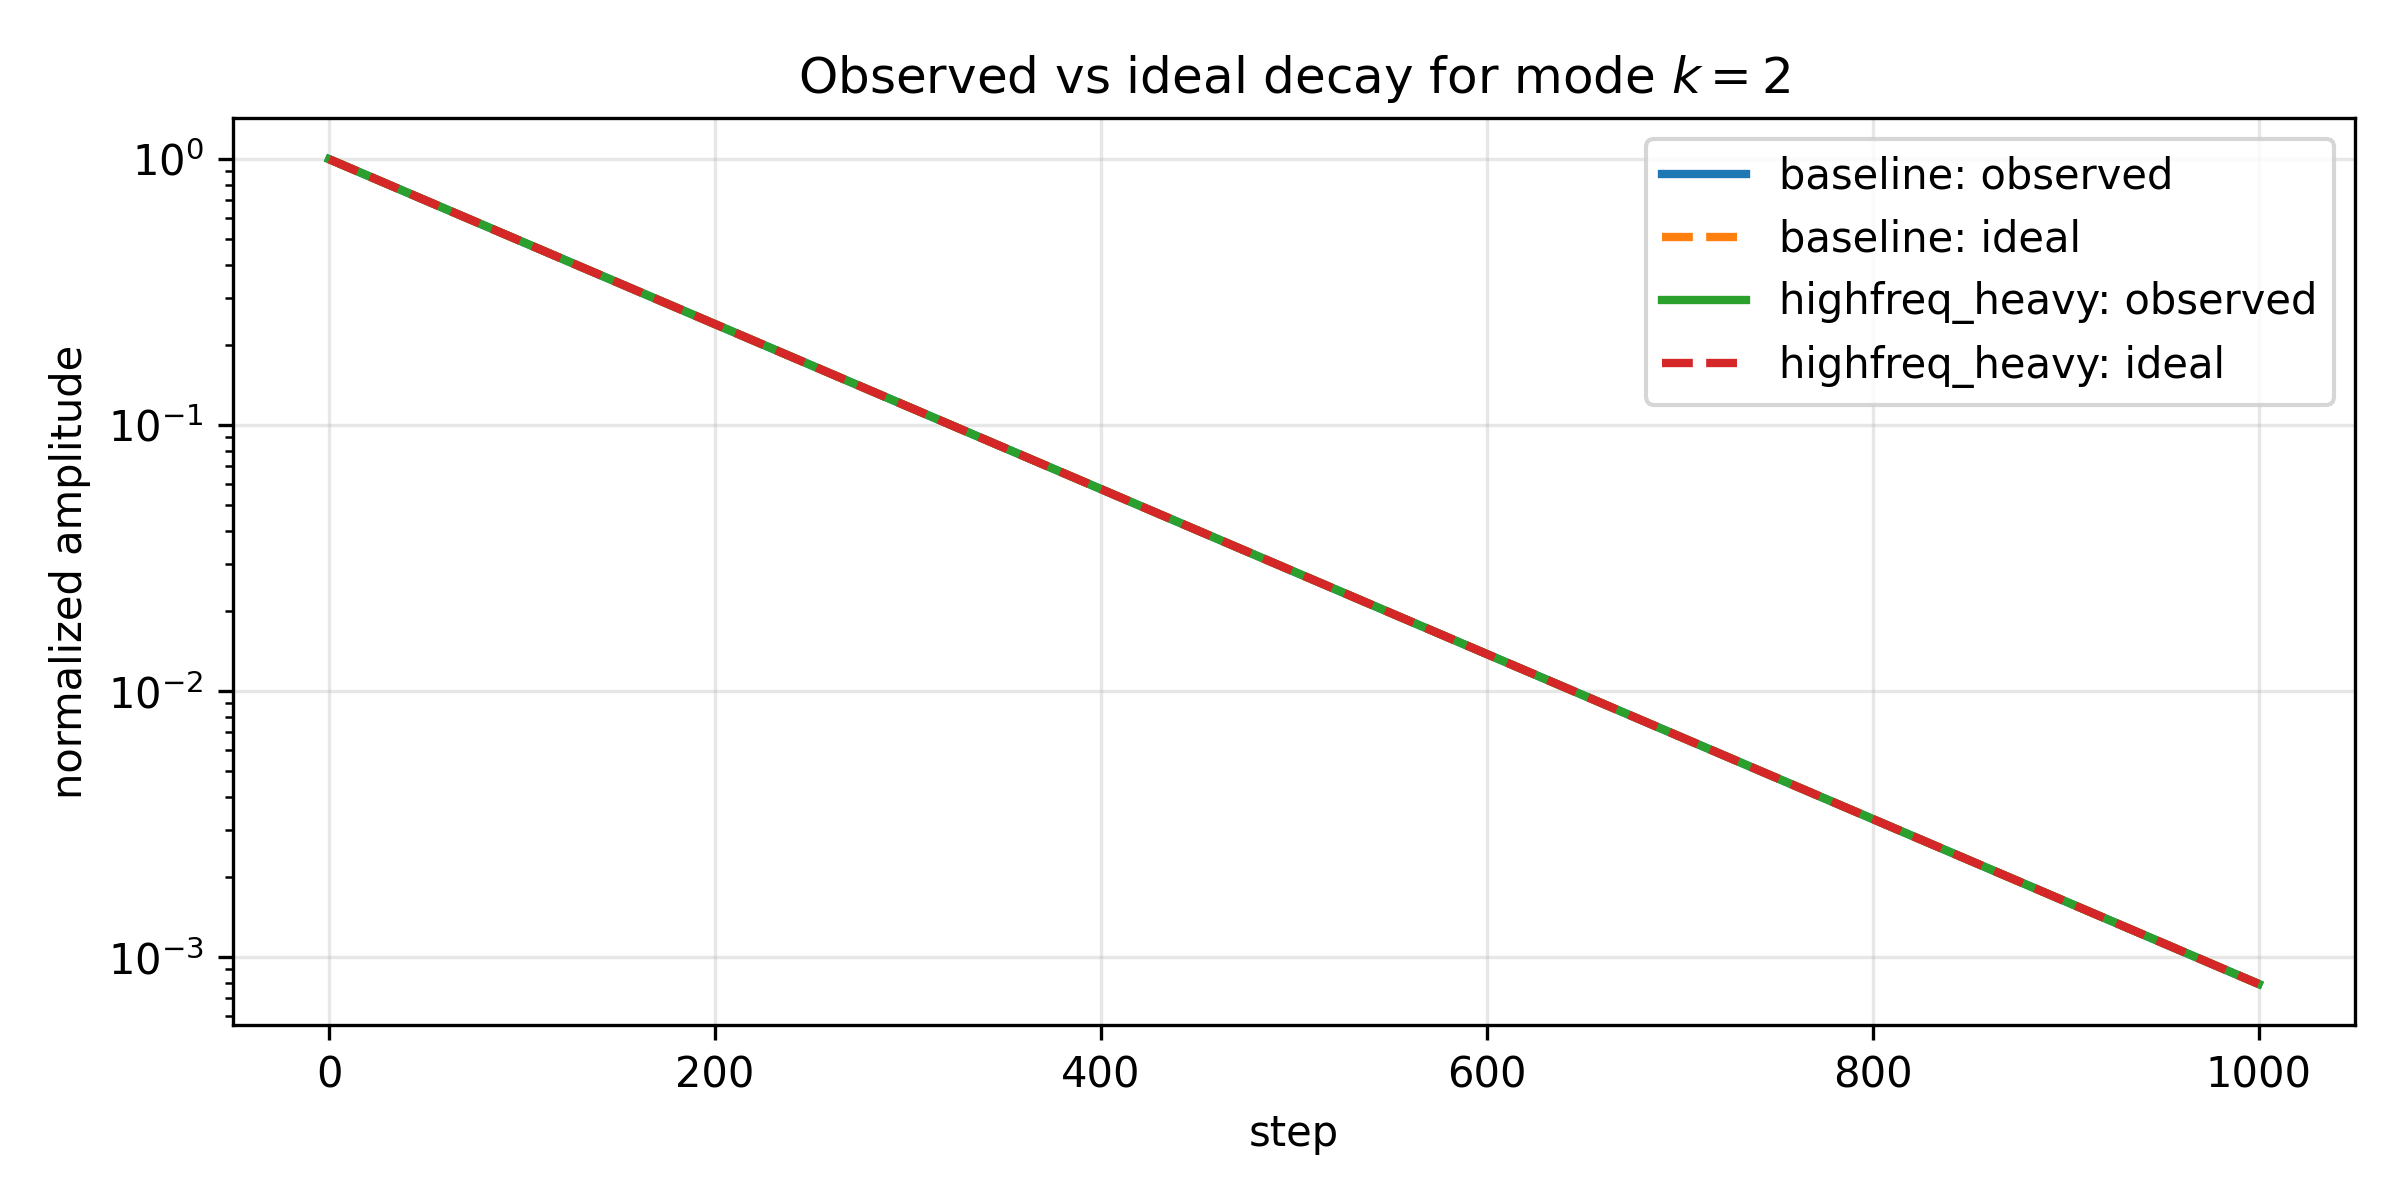
\includegraphics[width=\linewidth]{images/observed_vs_ideal_residual_decay_mode_2.png}
		\caption{Mode $k=2$}
	\end{subfigure}
	\hfill
	\begin{subfigure}[t]{0.48\textwidth}
		\centering
		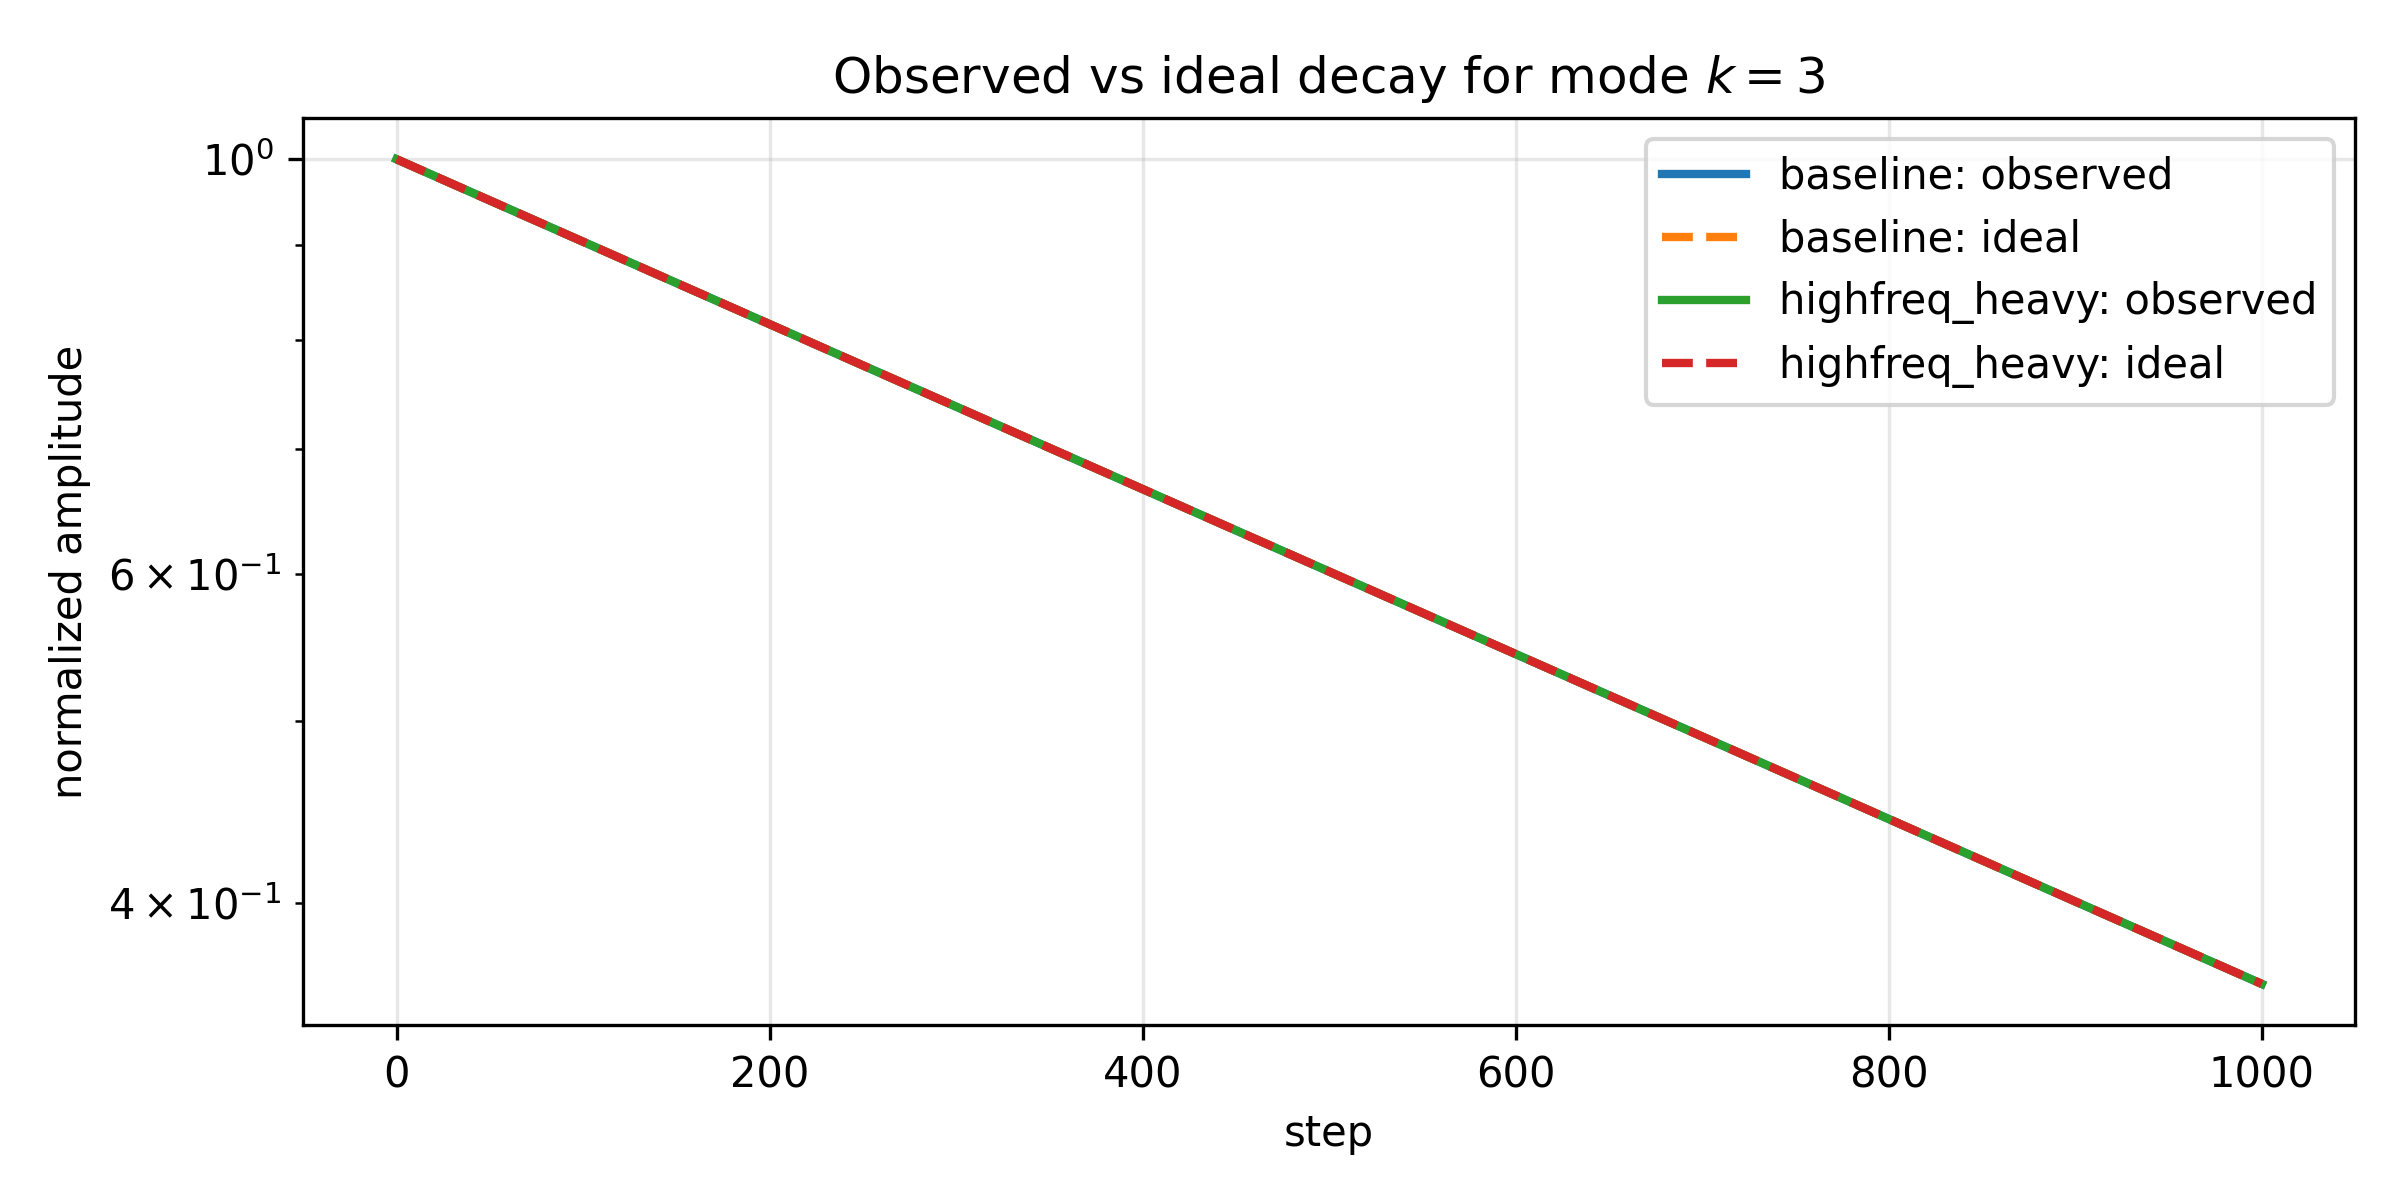
\includegraphics[width=\linewidth]{images/observed_vs_ideal_residual_decay_mode_3.png}
		\caption{Mode $k=3$}
	\end{subfigure}
	\caption{Observed versus ideal normalized residual decay for all active modes in the amplitude-swap experiment. Across the two targets, the normalized decay curves coincide, confirming that amplitudes do not change the decay rate.}
\end{figure}

\begin{figure}[H]
	\centering
	\begin{subfigure}[t]{0.48\textwidth}
		\centering
		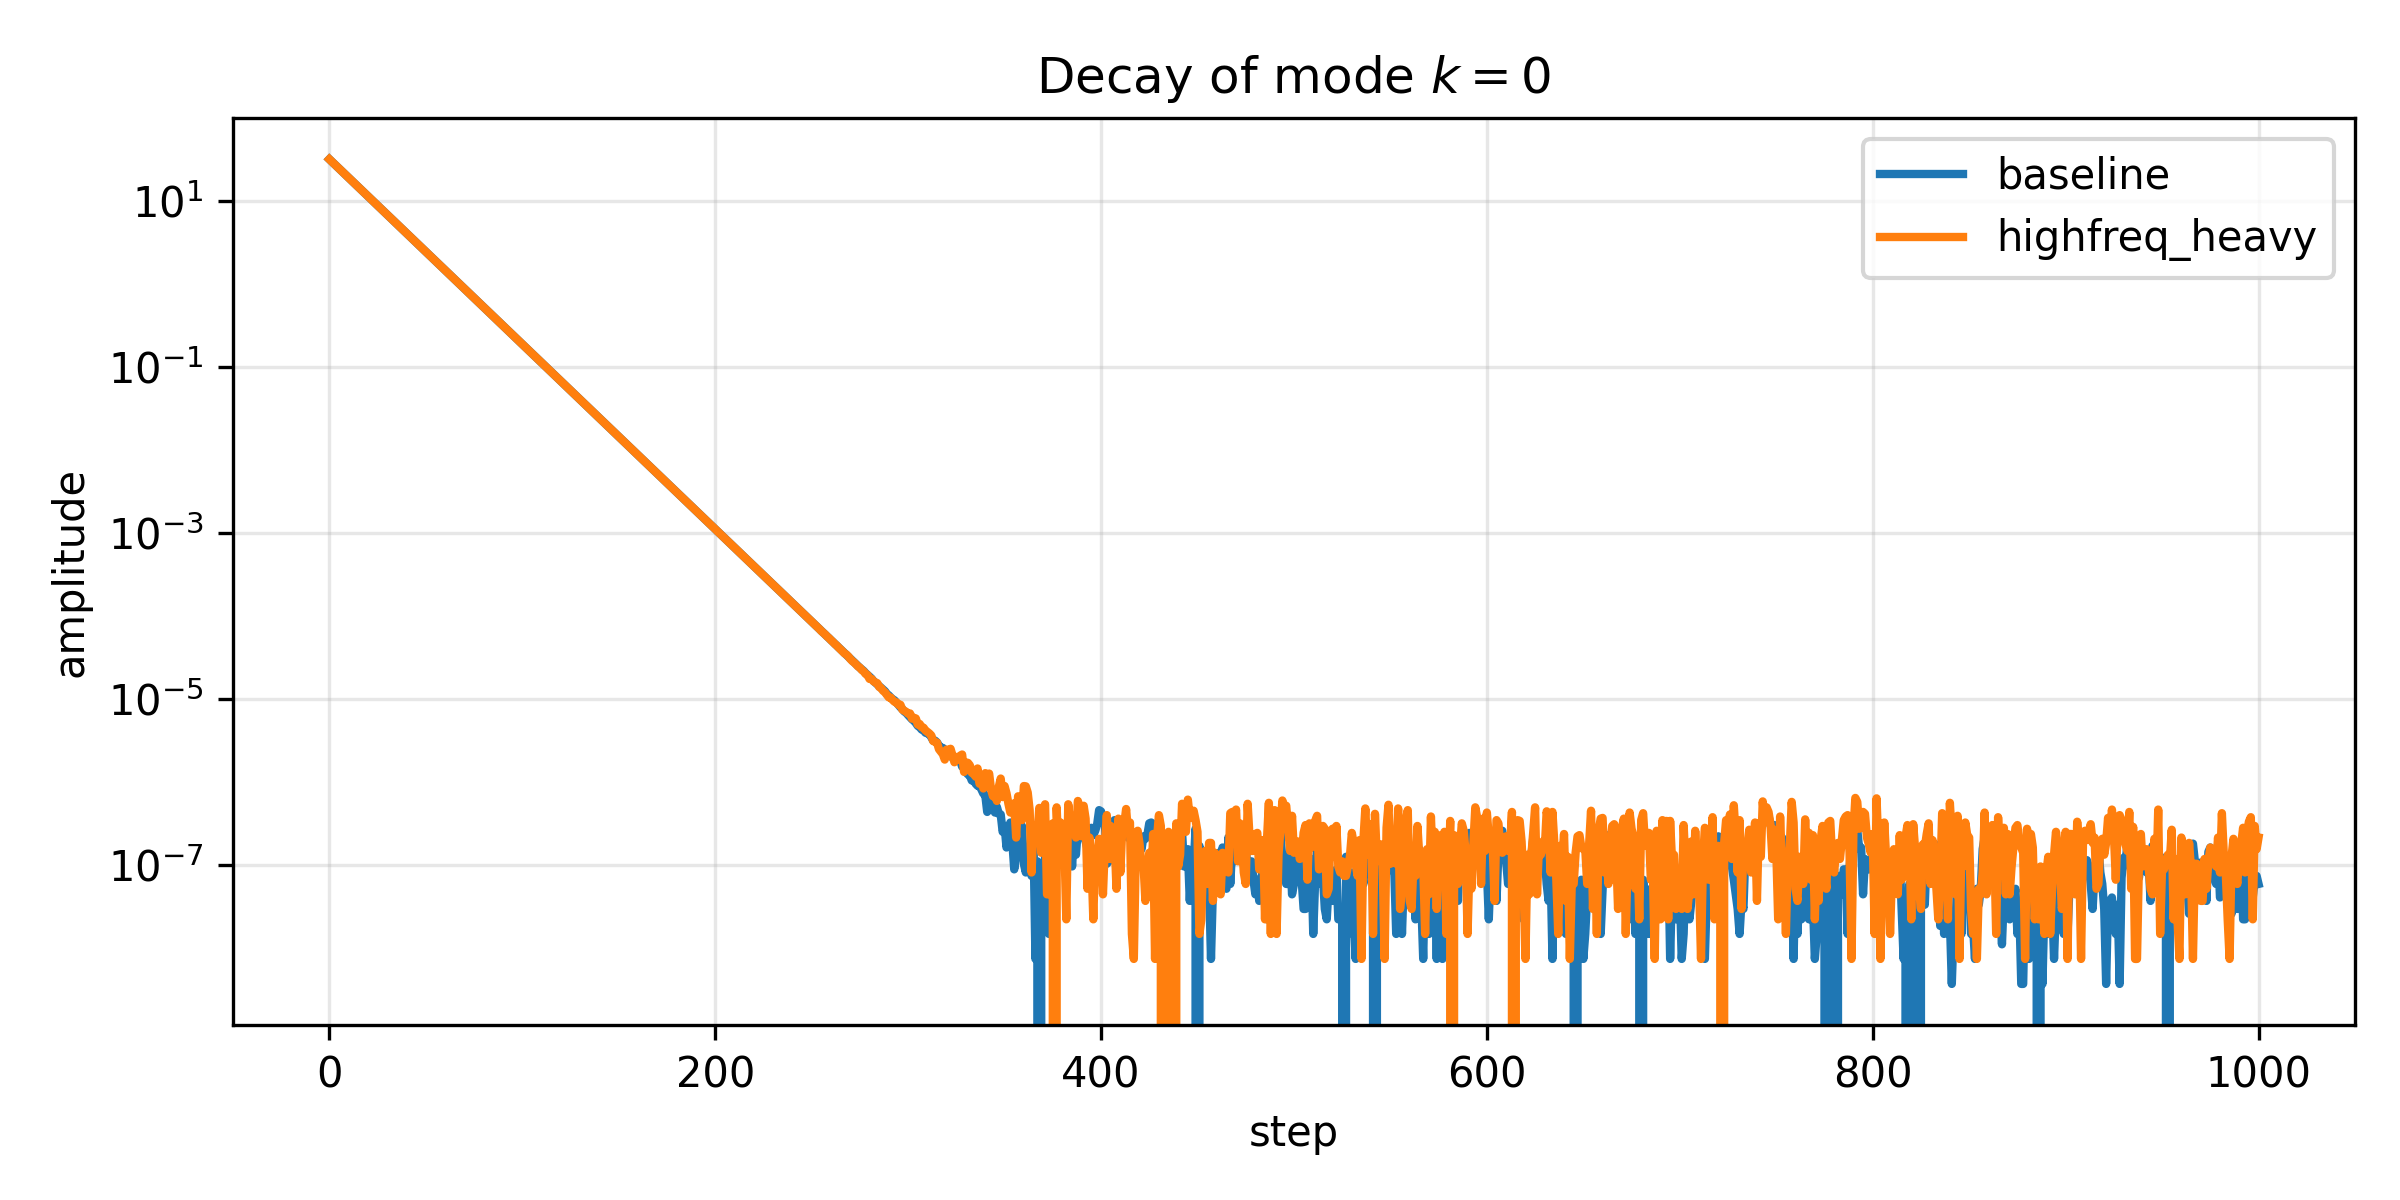
\includegraphics[width=\linewidth]{images/unnormalized_residual_decay_mode_0.png}
		\caption{Mode $k=0$}
	\end{subfigure}
	\hfill
	\begin{subfigure}[t]{0.48\textwidth}
		\centering
		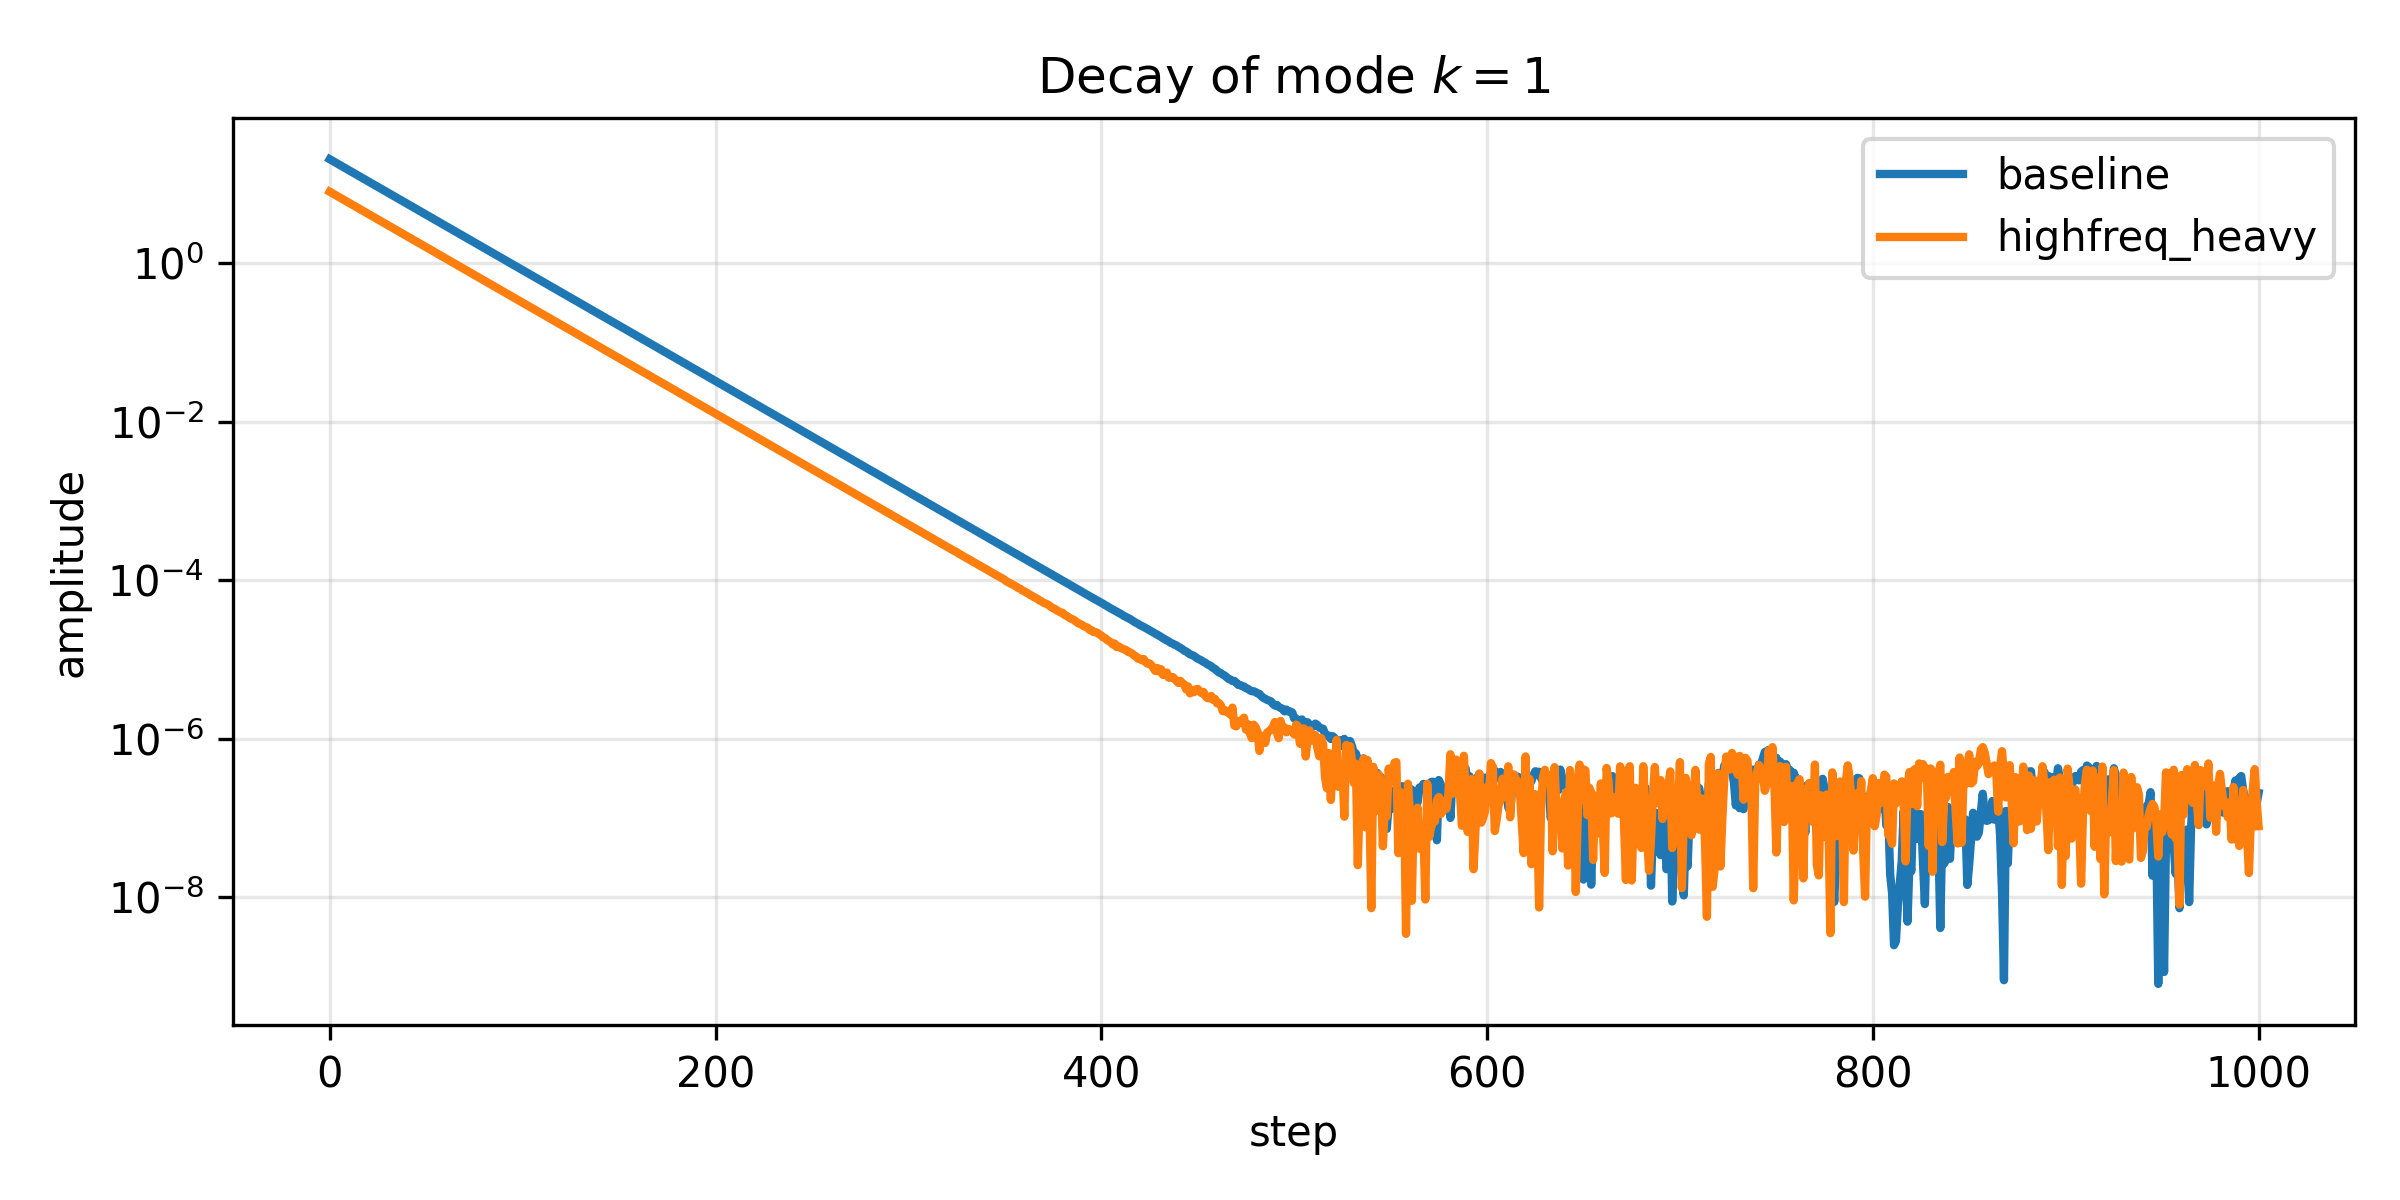
\includegraphics[width=\linewidth]{images/unnormalized_residual_decay_mode_1.png}
		\caption{Mode $k=1$}
	\end{subfigure}

	\vspace{0.6em}

	\begin{subfigure}[t]{0.48\textwidth}
		\centering
		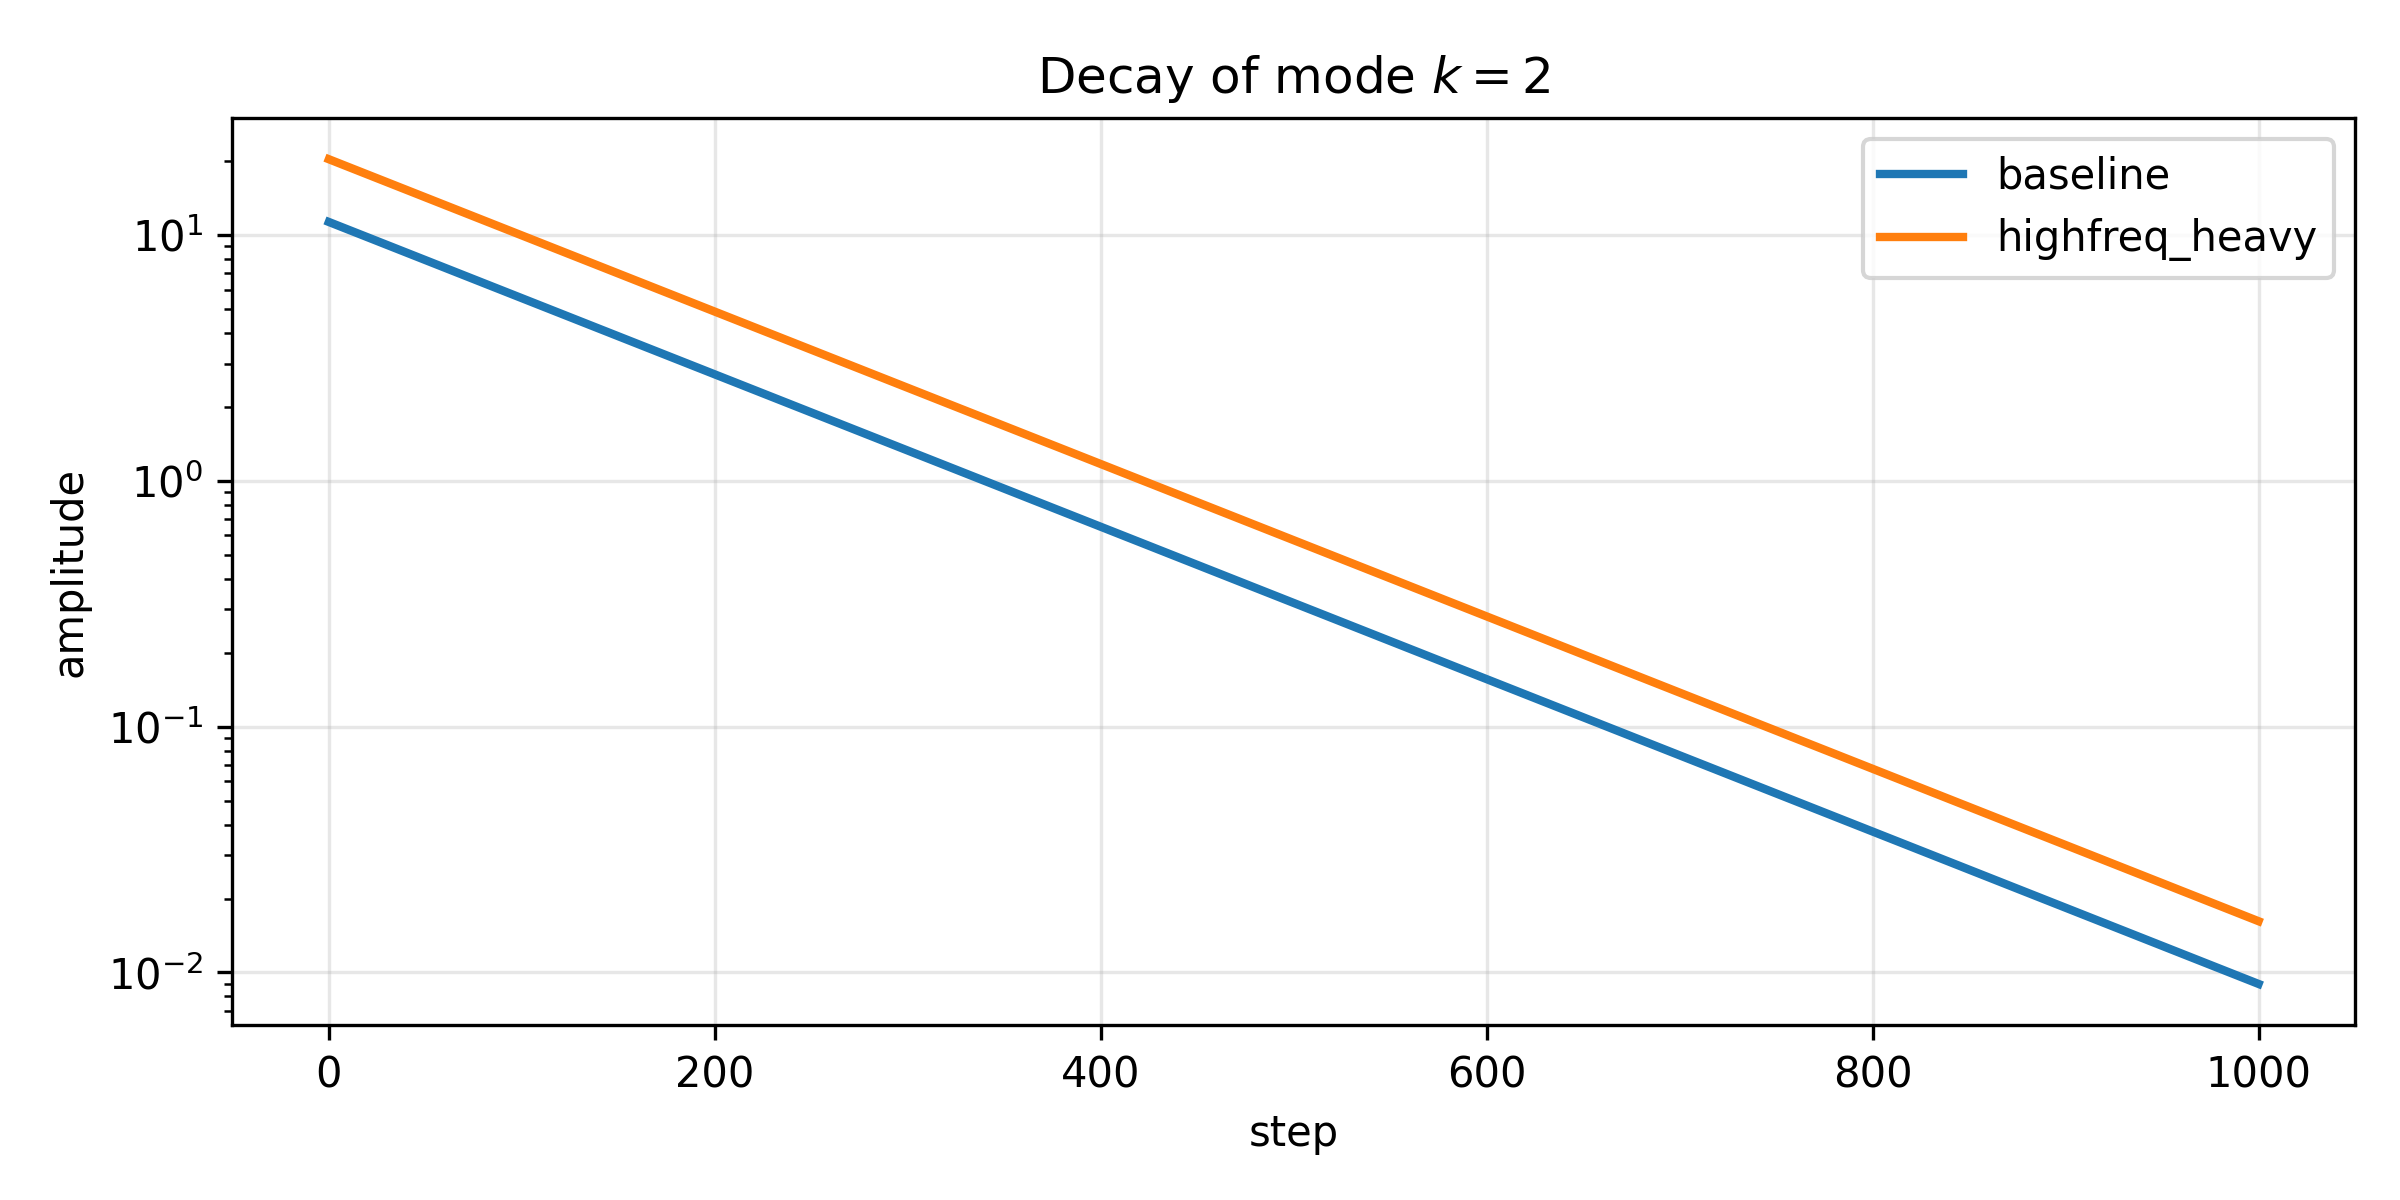
\includegraphics[width=\linewidth]{images/unnormalized_residual_decay_mode_2.png}
		\caption{Mode $k=2$}
	\end{subfigure}
	\hfill
	\begin{subfigure}[t]{0.48\textwidth}
		\centering
		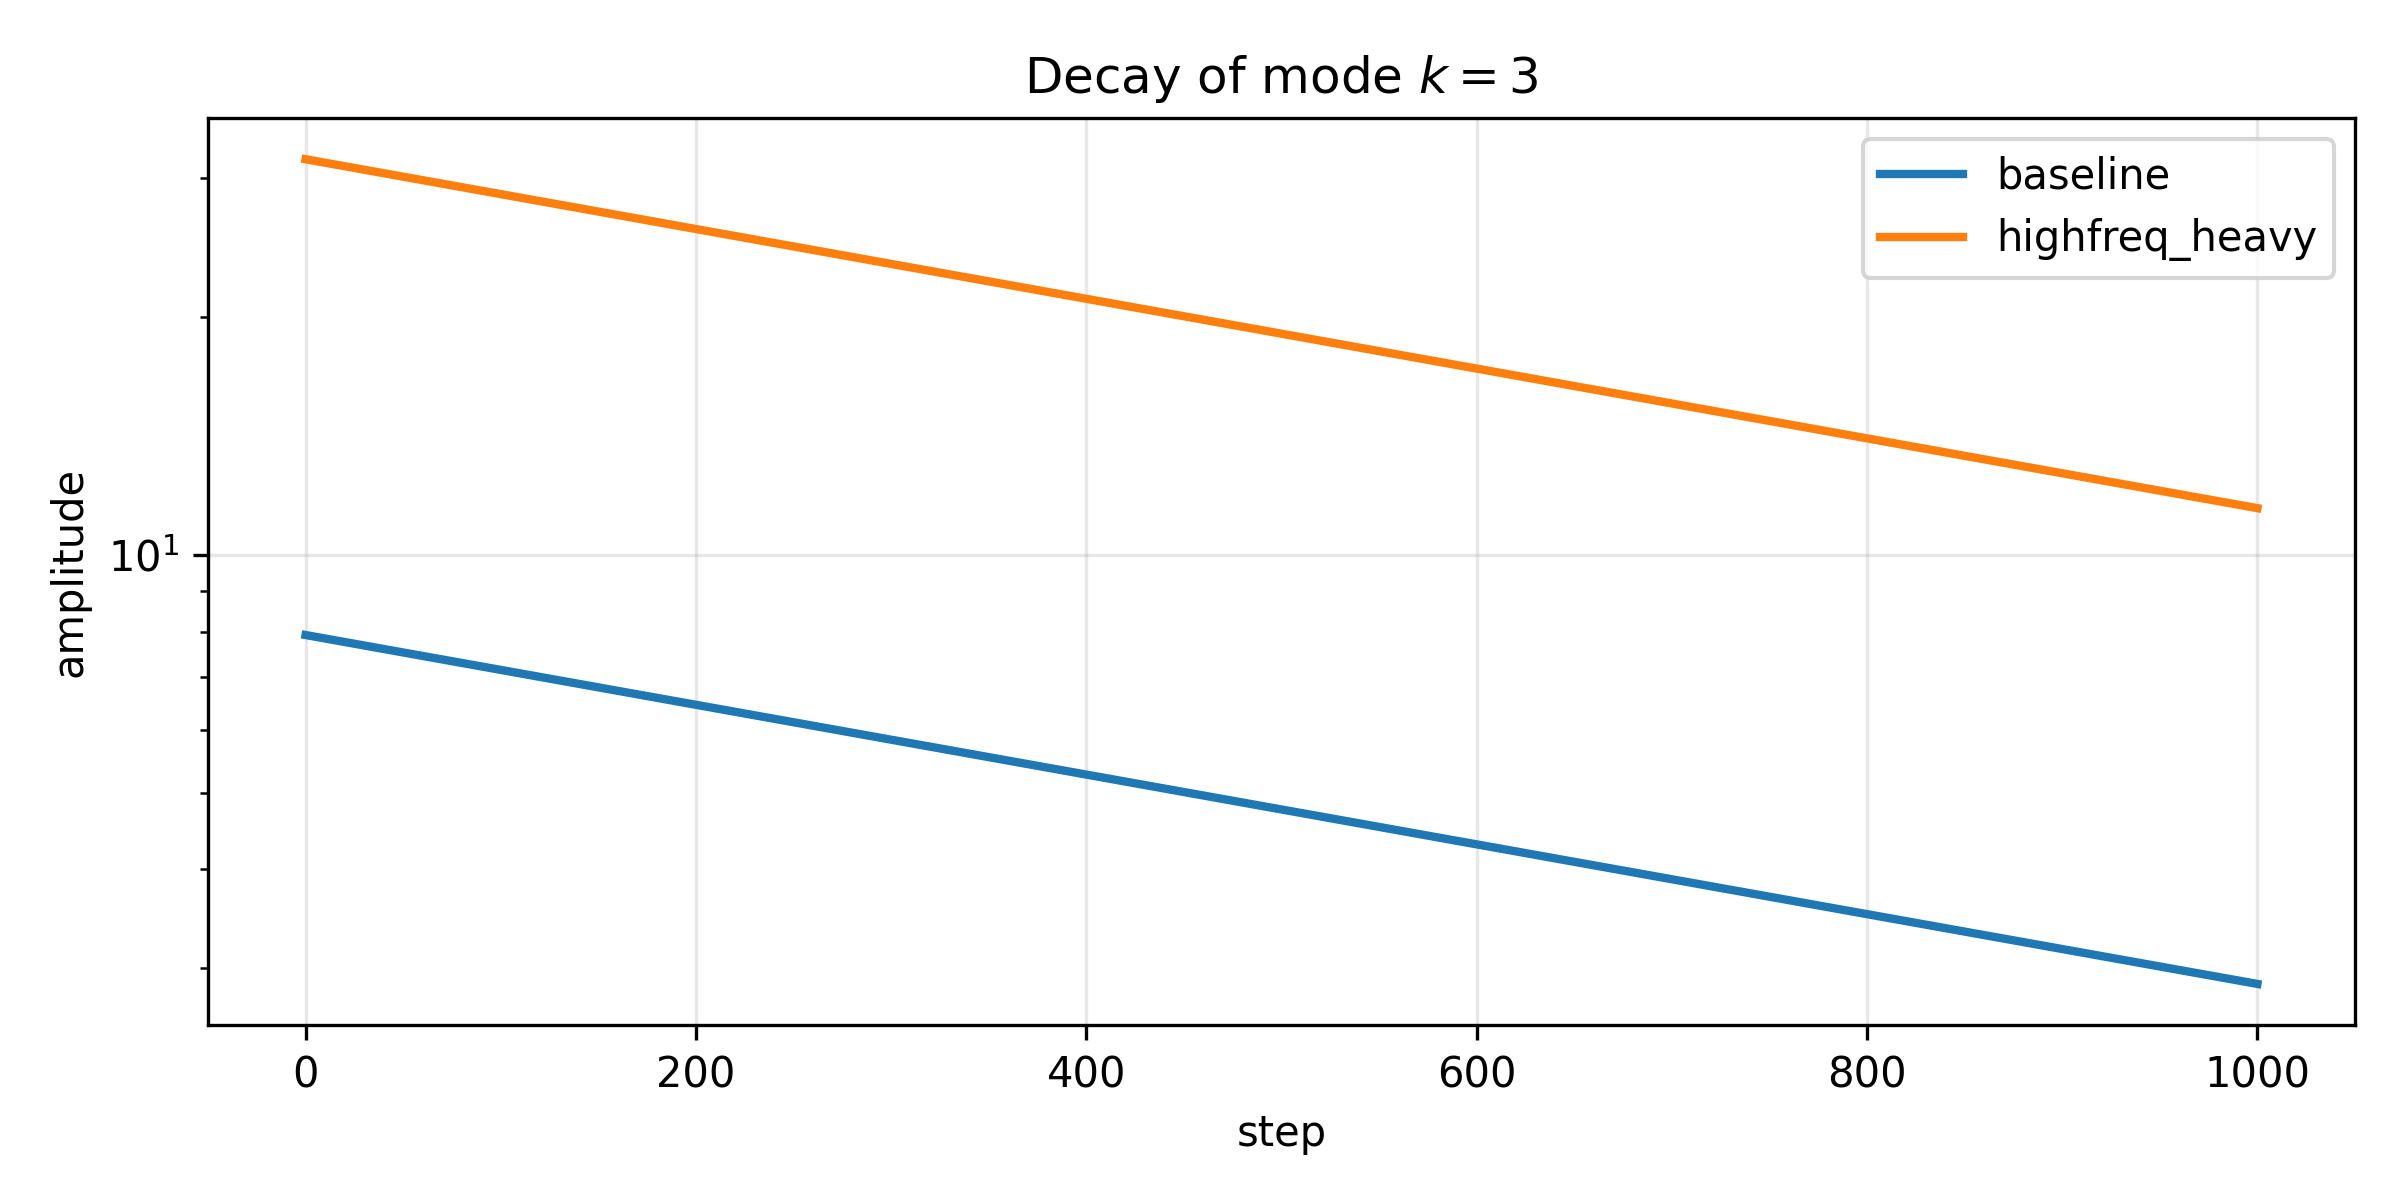
\includegraphics[width=\linewidth]{images/unnormalized_residual_decay_mode_3.png}
		\caption{Mode $k=3$}
	\end{subfigure}
	\caption{Observed unnormalized residual decay for the amplitude-swap experiment. These plots retain the amplitude factor and therefore explain the difference in overall error between the two targets.}
\end{figure}
\end{document}
